\documentclass{article}

\usepackage[paper=a4paper,margin=0.9in]{geometry}

\usepackage{mathtools}
\usepackage{derivative}
\usepackage{graphicx}
\usepackage{enumitem} % enumeration label options
\usepackage{amsfonts} % \mathbb, ...
\usepackage{amssymb} % \subsetneq, \nmid, ...
\usepackage{stmaryrd} % \mapsfrom
\usepackage{yhmath} % \widehat
\usepackage{tikz-cd}
\usepackage{amsthm}
\usepackage{dynkin-diagrams}

\setlength{\parindent}{0pt}

\newtheorem*{conjecture}{Conjecture}
\newtheorem*{theorem}{Theorem}
\newtheorem*{lemma}{Lemma}
\newtheorem*{proposition}{Proposition}
\newtheorem*{corollary}{Corollary}
\newtheorem*{claim}{Claim}

\theoremstyle{definition}
\newtheorem*{definition}{Definition}
\newtheorem*{fact}{Fact}
\newtheorem*{example}{Example}
\newtheorem*{nonexample}{Non-Example}
\newtheorem*{remark}{Remark}
\newtheorem*{exercise}{Exercise}

\DeclareMathOperator{\Hom}{Hom}
\DeclareMathOperator{\Hol}{Hol}
\DeclareMathOperator{\End}{End}
\DeclareMathOperator{\Gr}{Gr}
\DeclareMathOperator{\Sp}{Sp}
\DeclareMathOperator{\SO}{SO}
\DeclareMathOperator{\SL}{SL}
\DeclareMathOperator{\GL}{GL}
\DeclareMathOperator{\im}{im}
\DeclareMathOperator{\tr}{tr}
\DeclareMathOperator{\gr}{gr}
\DeclareMathOperator{\rad}{rad}
\DeclareMathOperator{\sgn}{sgn}
\DeclareMathOperator{\rank}{rank}
\DeclareMathOperator{\Sym}{Sym}
\DeclareMathOperator{\Vect}{Vect}

\newcommand{\conj}[1]{\overline{#1}}

\newcommand{\id}{\mathrm{id}}
\newcommand{\cl}{\mathrm{cl}}
\newcommand{\an}{\mathrm{an}}
\newcommand{\sing}{\mathrm{sing}}
\newcommand{\ev}{\mathrm{ev}}
\newcommand{\dR}{\mathrm{dR}}
\newcommand{\CH}{\mathrm{CH}}
\newcommand{\Hdg}{\mathrm{Hdg}}
\newcommand{\FS}{\mathrm{FS}}

\renewcommand{\L}{\mathcal{L}}
\renewcommand{\O}{\mathcal{O}}
\newcommand{\E}{\mathcal{E}}
\newcommand{\U}{\mathcal{U}}
\renewcommand{\u}{\mathfrak{u}}
\newcommand{\m}{\mathfrak{m}}
\newcommand{\RP}{\mathbb{RP}}
\newcommand{\CP}{\mathbb{CP}}
\newcommand{\F}{\mathbb{F}}
\renewcommand{\H}{\mathbb{H}}
\newcommand{\bbO}{\mathbb{O}}
\renewcommand{\P}{\mathbb{P}}
\newcommand{\A}{\mathbb{A}}
\newcommand{\N}{\mathbb{N}}
\newcommand{\Z}{\mathbb{Z}}
\newcommand{\Q}{\mathbb{Q}}
\newcommand{\R}{\mathbb{R}}
\newcommand{\C}{\mathbb{C}}

\title{Topics in Geometry (LSGNT) - Notes and Exercises}
\author{Calum Crossley}
\date{2023-2024}

\begin{document}

\maketitle

\section{Spec and Proj - Ed Segal}

\subsection*{Exercise solutions}

% TODO: Include question statements

\begin{enumerate}

\item
\begin{enumerate}[label=(\alph*)]

\item 
A decomposition $V=V_1\cup V_2$ into subvarieties (Zariski
closed sets) $V_1$ and $V_2$ is the same thing as a pair of
disjoint Zariski open sets $V\setminus V_1$ and
$V\setminus V_2$. The decomposition is non-trivial iff the open
sets are non-empty.

\item
If $fg=0$ in $\C[V]$ then $V=V(f)\cup V(g)$, so irreducibility
implies one of $V(f)$ or $V(g)$ is $V$, meaning one of $f$ or
$g$ is zero. Hence $\C[V]$ is an integral domain if $V$ is
irreducible.

If $V=V_1\cup V_2$ and $V_i\ne V$ then some polynomial
$f_i$ vanishes on $V_i$ but not $V$, otherwise the equations
defining $V_i$ would include all of $V$. Then $f_1f_2$ vanishes
on $V_1\cup V_2=V$, so $\C[V]$ has zero-divisors.

\end{enumerate}

\item
\begin{enumerate}[label=(\alph*)]

\item 
Let $f$ be a non-constant polynomial with no roots over a non-algebraically
closed field, such as $x^2+1$ over $\R$. Then $V(f)=\emptyset$ so
$I_{V(f)}=(1)$, but $1\notin\rad(f)$ as $f$ is non-constant.

\item
Over $\F_p$ affine space $\A^n$ has finitely many points, so $I_{\A^n}$ consists
of the polynomials vanishing at these points, including for example
$\prod_{a_1\in\F_p}(x_1-a_1)=x_1^p-x_1$. We have
\begin{align*}
    I_{\A^n(\F_p)}
        &= \bigcap_{a_1,\ldots,a_n\in\F_p}(x_1-a_1,\ldots,x_n-a_n) \\
        &= \bigcap_{a_2,\ldots,a_n\in\F_p}(x_1^p-x_1,x_2-a_2,\ldots,x_n-a_n) \\
        &= (x_1^p-x_1,\ldots,x_n^p-x_n).
\end{align*}

\end{enumerate}

\item
Consider the affine variety $X=V(x_{n+1}f-1)\subseteq\A^{n+1}$. We have a
morphism $X\to\A^n\setminus V(f)$ by projection:
$(a_1,\ldots,a_{n+1})\mapsto(a_1,\ldots,a_n)$, since
$a_{n+1}f(a_1,\ldots,a_n)=1$ implies $f(a_1,\ldots,a_n)\ne0$. This has an
inverse given by $(a_1,\ldots,a_n)\mapsto(a_1,\ldots,a_n,1/f(a_1,\ldots,a_n))$,
which is also regular.

\item
Suppose $V\subseteq\A^n$ and $W\subseteq\A^m$ correspond to quotient maps
$\C[x_1,\ldots,x_n]\to\C[V]$ and $\C[y_1,\ldots,y_m]\to\C[W]$. Choose a
lift of $\C[W]\to\C[V]$ and let $f_1,\ldots,f_m\in\C[x_1,\ldots,x_n]$
be the images of $y_1,\ldots,y_m$, as in the following diagram.
\begin{equation*}
\begin{tikzcd}[column sep=huge]
    &\C[W] \ar[r] &\C[V] \\
    &\C[y_1,\ldots,y_m] \ar[u,two heads] \ar[r,dashed,"f_1{,}\ldots{,}f_m"]
    &\C[x_1,\ldots,x_n] \ar[u,two heads]
\end{tikzcd}
\end{equation*}
Then $(x_1,\ldots,x_n)\mapsto(f_1,\ldots,f_m)$ is a morphism $\A^n\to\A^m$, and
since $I_W$ maps to $I_V$ in the diagram, it restricts to a morphism $V\to W$.
Moreover the pullback $\C[V]\to\C[W]$ given by composition with this map
precisely corresponds to substituting $f_1,\ldots,f_m$ for $y_1,\ldots,y_m$, so
from the diagram we recover the original homomorphism $\C[W]\to\C[V]$.

\item
If $\varphi:\C[V]\to\C[x]/(x^2)$ we have $\C[V]\to\C[x]/(x^2)\to\C[x]/(x)=\C$,
and the kernel of this map is a maximal ideal
$\m_p=\varphi^{-1}((x))\subseteq\C[V]$ corresponding to a point $p\in V$.
Moreover $\m_p/\m_p^2$ maps to $(x)/(x^2)=\C\cdot x$, giving an element of the
dual $(\m_p/\m_p^2)^\vee$ of $\m_p/\m_p^2$ considered as a
$\C[V]/\m_p=\C$-vector space.

\textbf{Claim 1:}
The data of a maximal ideal $\m_p\subseteq\C[V]$ and a functional
$v\in(\m_p/\m_p^2)^\vee$ determines a unique homomorphism $\C[V]\to\C[x]/(x^2)$
respecting the above construction.

\textbf{Proof:}
Define $\C[V]\to\C[x]/(x^2)$ by $f\mapsto f(p)+v(f-f(p))x$. This is clearly
$\C$-linear, and respects products since
\begin{equation*}
    fg-f(p)g(p) \equiv f(p)(g-g(p)) + g(p)(f-f(p)) \mod \m_p^2;
\end{equation*}
the difference being $(f-f(p))(g-g(p))$. By construction the preimage of $(x)$
is $\m_p$, and the induced map $\m_p/\m_p^2\to(x)/(x^2)=\C\cdot x$ is indeed
given by $v$.

\textbf{Claim 2:}
The space $(\m_p/\m_p^2)^\vee$ is canonically identified with the tangent space
to $V$ at $p$.

\textbf{Proof:}
Inuitively, elements of $(\m_p/\m_p^2)^\vee$ are functionals insensitive to
second order vanishing, which are first order differential operators;
differentiation along tangent vectors. Suppose $V=V(f_1,\ldots,f_r)$ in $\A^n$.
Then the tangent space to $V$ at $p$ should be given by
\begin{equation*}
    T_pV = \left\{(v_1,\ldots,v_n)\in\C^n
        : v_1\pdv{f_i}{x_1}(p)+\cdots+v_n\pdv{f_i}{x_n}(p)=0
        \text{ for $i=1,\ldots,r$}\right\}.
\end{equation*}
We define $\psi:(\m_p/\m_p^2)^\vee\to T_pV$ by
$v\mapsto(v(x_1-p_1),\ldots,v(x_n-p_n))$; evaluating the operator on
coordinates. This is well-defined since
\begin{equation*}
    (x_1-p_1)\pdv{f_i}{x_1}(p) + \cdots + (x_n-p_n)\pdv{f_i}{x_n}(p)
        \equiv f_i \mod \m_p^2,
\end{equation*}
and $f_i=0$ in $\C[V]$. It has an inverse given by
\begin{equation*}
    (v_1,\ldots,v_n) \mapsto
        \left(f\mapsto v_1\pdv{f}{x_1}(p)+\cdots+v_n\pdv{f}{x_n}(p)\right),
\end{equation*}
which is well-defined since elements of $\m_p^2$ map to zero by the product
rule, and multiples of $f_1,\ldots,f_r$ map to zero by the product rule and the
fact that $(v_1,\ldots,v_n)\in T_pV$. That this is indeed an inverse follows
from the fact that
\begin{equation*}
    (x_1-p_1)\pdv{f}{x_1}(p) + \cdots + (x_n-p_n)\pdv{f}{x_n}(p)
        \equiv f \mod \m_p^2.
\end{equation*}

\item
The corresponding homomorphism of coordinate rings $\C[x,y]/(y^2-x^3)\to\C[t]$
given by $x\mapsto t^2$, $y\mapsto t^3$ is not an isomorphism, since
$\C[t^2,t^3]\subsetneq\C[t]$.

However we have a set-theoretic inverse:
\begin{equation*}
    (x,y)\mapsto\begin{dcases*}
        x/y & if $y\ne0$ \\
        0 & otherwise.
    \end{dcases*}
\end{equation*}
Adjoining a point at infinity to both curves we get compact Hausdorff spaces in
the complex topology, so this inverse is even continuous with respect to the
complex topology.

\item
For $U_0\cap U_1$ we have $[1,x_1,x_2]=[1/x_1,1,x_2/x_1]$, giving
$(x_1,x_2)\mapsto(1/x_1,x_2/x_1)$.

For $U_0\cap U_2$ we have $[1,x_1,x_2]=[1/x_2,x_1/x_2,1]$, giving
$(x_1,x_2)\mapsto(1/x_2,x_1/x_2)$.

For $U_1\cap U_2$ we have $[x_0,1,x_2]=[x_0/x_2,1/x_2,1]$, giving
$(x_0,x_2)\mapsto(x_0/x_2,1/x_2)$.

\item
Suppose $f\in\C[x_1,\ldots,x_n]$ defines a hypersurface $V=V(f)\subseteq\A^n$.
We obtain a homogeneous polynomial $\hat f\in\C[x_1,\ldots,x_{n+1}]$ by
\begin{equation*}
    \hat f = x_{n+1}^{\deg f}\cdot f(x_1/x_{n+1},\ldots,x_n/x_{n+1}),
\end{equation*}
giving a projective hypersurface in $\P^n$ whose intersection with the affine
part $x_{n+1}\ne0$ is $V(f)$. It is in fact the closure of this affine part in
$\P^n$, since substituting $x_{n+1}=1$ and applying this process to a
homogeneous polynomial recovers the original polynomial up to a multiple of
$x_{n+1}$. When the codimension is higher homogenizing the generators of the
defining ideal like this is insufficient to cut out the projective closure; one
must homogenize all elements of the vanishing ideal. For example homogenizing
the generators of $V(x_1-x_2^2,x_1-x_3^3)$ gives
$V(x_1x_4-x_2^2,x_1x_4^2-x_3^3)$, whose points at infinity are given by

\item
\begin{enumerate}[label=(\alph*)]

\item 
Define a map $\P^1\to C$ by $[s:t]\mapsto[s^2:t^2:st]$. Now $xy=z^2$ implies
$[y:z]=[z:x]$ when both are defined, so $[x:y:z]\mapsto[y:z]$ and
$[x:y:z]\mapsto[z:x]$ glue to give an inverse $C\to\P^1$.

\item
Matrices of rank 1 are non-zero, and the rank is preserved by non-zero scalar
multiplication. Non-zero traceless $2\times2$ matrices are parametrized up to
scale by $\P^2$ as follows:
\begin{equation*}
    [x:y:z] \mapsto \begin{pmatrix}
        z & -x \\ y & -z
    \end{pmatrix},
\end{equation*}
and the rank is 1 iff the determinant $xy-z^2$ vanishes. Hence $C$ parametrizes
rank 1 traceless $2\times2$ matrices up to scale. From (a) we also get a
parametrization by $\P^1$:
\begin{equation*}
    [s:t] \mapsto \begin{pmatrix}
        st & -s^2 \\ t^2 & -st
    \end{pmatrix}.
\end{equation*}

\item
Over $\C$ the quadratic forms are determined up to equivalence by rank, so
replacing $xy-z^2$ by a non-degenerate quadratic form results in a curve
isomorphic to $C\cong\P^1$. A quadratic form of rank 2 results in a curve
isomorphic to $V(xy)$; two lines, and a quadratic form of rank 1 results in a
curve isomorphic to $V(x^2)$; one line (or a scheme-theoretic double line).

Different quadratic forms correspond to different special matrix forms as in
(b), for example
\begin{equation*}
    x^2 + y^2 = \det\begin{pmatrix}
        x & -y \\
        y & x
    \end{pmatrix}
\end{equation*}
and
\begin{equation*}
    xw - yz = \det\begin{pmatrix}
        x & y \\ z & w
    \end{pmatrix}.
\end{equation*}
The latter gives the Segre embedding $\P^1\times\P^1\to\P^3$,
$(X_1:X_2,Y_1:Y_2)\mapsto(X_1Y_1:X_1Y_2:X_2Y_1:X_2Y_2)$, whose image is
$V(XW-YZ)$.

\end{enumerate}

\item
\begin{enumerate}[label=(\alph*)]

\item
For $\epsilon\ne0$ we have $V_\epsilon\cong\A^1\setminus\{0\}$ via
$z\mapsto(z,\epsilon/z)$, which is
$(re^{i\theta},\epsilon r^{-1}e^{-i\theta})$
in polar coordinates. This forms a cylinder joining up the two real arcs
$\theta=0$ and $\theta=\pi$, with $(x,y)$ connecting to $(-x,-y)$ on the circle
$r=|x|$.

% TODO: picture

If we follow the circles $r=c$ for constant $c$ as $\epsilon\to0$ we get the
circles around the origin of the $x$-plane in $xy=0$. Similarly the circles
$r=c\epsilon$ converge to the circles around the origin of the $y$-plane.
Meanwhile the circle $r=\sqrt{|\epsilon|}$ contracts to the origin, so the
cylinder is pinched into two planes / discs connected at the origin.

\item % TODO

\end{enumerate}

\end{enumerate}

\newpage

\section{Poincar\'e duality - Steven Sivek}

Recommended source: Bott \& Tu, Differential Forms in Algebraic Topology.

\subsection*{Rough idea}

Take a (smooth, oriented) manifold $M^n$. Compact (smooth, oriented) submanifolds
$X^k,Y^{n-k}\subseteq M$ intersect \emph{transversely} at $p\in X\cap Y$ if we
have
\begin{equation*}
    T_pX\oplus T_pY = \pm T_pM,
\end{equation*}
where the sign matches the orientation on the LHS induced from $X$ and $Y$ with
the orientation of $M$. Write $\sgn(p)$ for this sign, and define the
\emph{intersection number}
\begin{equation*}
    i(X,Y) = \sum_{p\in X\cap Y}\sgn(p).
\end{equation*}

\begin{claim}
    This only depends on $[X]\in H_k(M)$, $[Y]\in H_{n-k}(M)$. Hence we get a
    bilinear form
    \begin{equation*}
        i:\frac{H_k(M)}{\text{torsion}}
            \otimes\frac{H_{n-k}(M)}{\text{torsion}}\to\Z.
    \end{equation*}
    (We can mod out by torsion since $\Z$ is torsion-free.)
\end{claim}

\begin{theorem}[Poincar\'e duality]
    This form is non-degenerate; if $i(X,Y)=0$ for all $Y$ then $X=0$.
\end{theorem}

\begin{corollary}
    We have $\rank H_k(M)=\rank H_{n-k}(M)$ for each $k$.
\end{corollary}

Suppose $\dim M=2m$. We get a pairing on $H_m(M)/\text{torsion}$, and this is
symmetric or anti-symmetric if $m$ is even or odd respectively (think about the
orientation of $T_pX\oplus T_pY$ vs. $T_pY\oplus T_pX$). Then Poincar\'e duality
says that this pairing is \emph{uni-modular}; the matrix representing it in an
integral basis has determinant $\pm1$.

The algebraic structure $(H_m(M),i)$ is an invariant of $M$. When $\dim M=4$ we
define the \emph{signature} $\sigma(M)$ to be the signature of this bilinear
form.

\begin{theorem}
    $\sigma(M)$ is a complete bordism invariant of oriented 4-manifolds.
\end{theorem}

\begin{theorem}[Donaldson]
    If $M^4$ is smooth, and $i_M$ is negative-definite, then $i_M$ is
    diagonalizable over $\Z$; given by $-I$ in some integral basis for $H_2(M)$.
\end{theorem}

\begin{theorem}[Freedman]
    There exists a topological manifold $M^4$ with $i_M=E_8$, which is
    negative-definite but not diagonalizable over $\Z$. Hence $M$ has no smooth
    structure.
\end{theorem}

(The form $E_8$ is defined on $\Z^8$ by the adjacency matrix for the Dynkin
diagram \dynkin{E}{8}.)

\subsection*{de Rham cohomology}

\begin{definition}
    A \emph{$k$-form} on $M$ is a section of $\Lambda^kT^*M$. That is, at every
    point a multilinear alternating form
    $\alpha_p:\underbrace{T_pM\otimes\cdots\otimes T_pM}_{\text{$k$ times}}\to\R$.
\end{definition}

The space $\Omega^k(M)$ of $k$-forms has extra structure:
\begin{itemize}
    \item Wedge product $\wedge:\Omega^k(M)\otimes\Omega^l(M)\to\Omega^{k+l}(M)$
    \item Exterior derivative $d:\Omega^k(M)\to\Omega^{k+1}(M)$
\end{itemize}
satisfying
\begin{itemize}
    \item $\alpha\wedge\beta=(-1)^{|\alpha|\cdot|\beta|}\beta\wedge\alpha$
    \item $d(\alpha\wedge\beta)
        = d\alpha\wedge\beta+(-1)^{|\alpha|}\alpha\wedge d\beta$ (Leibniz rule)
    \item $d^2=0$.
\end{itemize}
This is the structure of a differential graded algebra, which is nice.

On $\R^n$, these operations are defined as follows:
\begin{itemize}
    \item $\Omega^k(\R^n)=\R\cdot\{fdx_{i_1}\wedge\cdots\wedge dx_{i_k}\}$,
        where $dx_i(\pdv{}{x_j})=\delta_{ij}$.

    \item $(fdx_{i_1}\wedge\cdots\wedge dx_{i_k})
                \wedge(gdx_{j_1}\wedge\cdots\wedge dx_{j_l})
            = fgdx_{i_1}\wedge\cdots\wedge dx_{i_k}
                \wedge dx_{j_1}\wedge\cdots\wedge dx_{j_l}$.

    \item $d(fdx_{i_1}\wedge\cdots\wedge dx_{i_k})
        = (\sum_i\pdv{f}{x_i}dx_i)\wedge dx_{i_1}\wedge\cdots\wedge dx_{i_k}$.
\end{itemize}
The general case is defined by patching these together from local coordinate
charts.

\begin{definition}
    A $k$-form $\alpha$ is \emph{closed} if $d\alpha=0$, and \emph{exact} if
    $\alpha=d\beta$ for some $(k-1)$-form $\beta$.

    The \emph{de Rham cohomology} is then
    \begin{equation*}
        H^k_\dR(M)
            = \{\text{closed $k$-forms}\}/\{\text{exact $k$-forms}\}
            = \ker d/\im d.
    \end{equation*}
\end{definition}

\begin{example}
    $\alpha\in\Omega^0(M)$ is a function, and locally
    $d\alpha=\sum_i\pdv{\alpha}{x_i}dx_i$, so $d\alpha=0$ iff $\alpha$ is
    locally constant. Hence $H^0_\dR(M)=\R$ if $M$ is connected.
\end{example}

\begin{example}
    If $k>\dim M$ then $\Omega^k(M)=0$ since $\Lambda^kT_pM=0$. Hence
    $H^k_\dR(M)=0$.
\end{example}

\begin{example}
    What is $H^1_\dR(\R)$? $\Omega^1(\R)=\{fdx:f:\R\to\R\}$ are all closed from
    above. Exact 1-forms are given by $dF=F'(x)dx$ for $F:\R\to\R$. Such an $F$
    with $dF=fdx$ always exists by the FTC, via
    \begin{equation*}
        F(x) = \int_0^xf(t)dt.
    \end{equation*}
    Hence $H^1_\dR(\R)=0$.
\end{example}

\begin{remark}
    By the Leibniz rule, the wedge product descends to cohomology, making
    $H^*_\dR(M)$ a graded-commutative $\R$-algebra.
\end{remark}

\begin{theorem}[Stokes' theorem]
    If $X^k\subseteq M^n$ is a compact submanifold with boundary, and
    $\alpha\in\Omega^{k-1}(M)$, we have
    \begin{equation*}
        \int_Xd\alpha = \int_{\partial X}\alpha.
    \end{equation*}
\end{theorem}

(Integration of forms is extended from $\R^n$ by patching.)

\begin{exercise}
    Show that there is a bilinear pairing
    \begin{equation*}
        H_k(M;\R)\otimes H^k_\dR(M)\to\R
    \end{equation*}
    given by
    \begin{equation*}
        [X^k]\otimes[\alpha]\mapsto\int_X\alpha.
    \end{equation*}
    (You may use a theorem of Thom, which states that after multiplying by a
    positive integer, any singular homology class of a manifold may be
    represented by a compact submanifold.)
\end{exercise}

\begin{proof}[Solution]
    For a homology class of the form $\frac{1}{n}[X^k]$ we define the image as
    \begin{equation*}
        \frac{1}{n}\int_X\alpha.
    \end{equation*}
    By the theorem of Thom on representability of multiples of homology classes
    this gives an output for all elementary tensors. It is well-defined, for if
    $\frac{1}{n}[X^k]=\frac{1}{m}[Y^k]$ then their difference is the boundary of
    some $(k+1)$-chain $c$, so
    \begin{equation*}
        \frac{1}{n}\int_X\alpha - \frac{1}{m}\int_Y\alpha
            = \int_{\partial c}\alpha
            = \int_cd\alpha
    \end{equation*}
    by Stokes' theorem, which is zero since $d\alpha=0$.
\end{proof}

\begin{lemma}[Poincar\'e lemma]
    \begin{equation*}
        H^k_\dR(\R^n) = \begin{dcases*}
            \R & $k=0$ \\
            0 & otherwise.
        \end{dcases*}
    \end{equation*}
\end{lemma}

\begin{proof}
    We induct on $n$. Assume $k>0$, and that all closed $k$-forms on $\R^n$ are
    exact. Consider a closed form $\omega\in\Omega^k(\R^{n+1})$. Taking
    coordinates $(x,t)$ on $\R^{n+1}=\R^n_x\times\R_t$, we may write
    $\omega=\alpha_t+dt\wedge\beta_t$ where $\alpha_t\in\Omega^k(\R^n)$ and
    $\beta_t\in\Omega^{k-1}(\R^n)$ for each $t$. Define
    $\eta_t=\int_0^t\beta_sds$, so that $\odv{}{t}\eta_t=\beta_t$. We have
    \begin{align*}
        d\eta_t
            &= d_x\eta_t + dt\wedge\odv{}{t}\eta_t \\
            &= d_x\eta_t + dt\wedge\beta_t,
    \end{align*}
    so $\omega-d\eta_t=\alpha_t-d_x\eta_t$. The LHS is closed, so
    $\alpha_t-d_x\eta_t$ is a closed form on $\R^n\times\R$, and in particular
    must be constant in $t$, given by some form in $\Omega^k(\R^n)$ which is
    exact by induction. Say $\alpha_t-d_x\eta_t=d_x\xi$, where
    $\xi\in\Omega^{k-1}(\R^n)$. Then $\omega=d\eta_t+d\xi$ is exact, where we
    pull back $\xi$ to $\R^n\times\R$ as a constant in $t$.
\end{proof}

There is an important variant of de Rham cohomology:
\begin{equation*}
    \Omega^k_c(M) = \{\text{compactly supported $k$-forms}\}
\end{equation*}
retains the differential graded algebra structure, and gives rise to compactly
supported (de Rham) cohomology
\begin{equation*}
    H^k_c(M) = \frac{\ker(d:\Omega^k_c(M)\to\Omega^{k+1}_c(M))}
        {\im(\Omega^{k-1}_c(M)\to\Omega^k_c(M))}.
\end{equation*}

\begin{remark}
    If $M$ is compact, then $\Omega^k_c(M)=\Omega^k(M)$ and
    $H^k_\dR(M)=H^k_c(M)$.
\end{remark}

\begin{example}
    $\ker(d:\Omega^0_c(\R^n)\to\Omega^1_c(\R^n))
    =\{\text{constant compactly supported functions}\}=0$, so $H^0_c(\R^n)=0$.
\end{example}

\begin{exercise}
    Prove $\alpha\in\Omega^1_c(\R)$ is exact iff $\int_\R\alpha=0$. Conclude
    that $H^1_c(\R)\cong\R$.
\end{exercise}

\begin{proof}[Solution]
    If $\alpha=df$ then $\int_\R\alpha=\int_\R df=0$ by Stokes' theorem.
    Conversely, if $\int_\R\alpha=0$ then the function
    \begin{equation*}
        f(t)=\int_{(-\infty,t)}\alpha
    \end{equation*}
    is zero for $t$ past the support of $\alpha$, as well as for $t$ preceding
    the support of $\alpha$, so $f\in\Omega^0_c(\R)$. By construction
    $\alpha=df$. This shows that integration gives an injection
    $H^1_c(\R)\to\R$, which is non-zero by the existence of bump functions, and
    therefore gives an isomorphism $H^1_c(\R)\cong\R$.
\end{proof}

\begin{lemma}[Poincar\'e lemma, pt 2]
    \begin{equation*}
        H^k_c(\R^n) = \begin{dcases*}
            \R & $k=n$ \\
            0 & otherwise.
        \end{dcases*}
    \end{equation*}
\end{lemma}

\subsection*{Poincar\'e duality}

\begin{theorem}[Poincar\'e duality]
    There is a perfect pairing
    \begin{align*}
        H^k_\dR(M)&\otimes H^{n-k}_c(M) \to \R \\
        [\alpha]&\otimes[\beta] \mapsto \int_M\alpha\wedge\beta.
    \end{align*}
    Equivalently, we have an isomorphism
    \begin{align*}
        H^k_\dR(M) &\to H^{n-k}_c(M)^* \\
        [\alpha] &\mapsto \int_M\alpha\wedge(-).
    \end{align*}
\end{theorem}

\begin{proof}[Proof sketch]
    Take a good cover of $M$; an open cover $\U=\{U_i\}$ such that
    finite intersections of the $U_i$ are contractible (or just discs). Induct
    on $|\U|$.
    \begin{itemize}
        \item $|\U|=1$: $M=\R^n$ so we use the Poincar\'e lemma; it is easy to
            check that the pairing is non-zero.

        \item Inductive step: Write $U=U_1\cup\cdots\cup U_{n-1}$, $V=U_n$, and
            look at the Mayer--Vietoris sequences for $M=U\cup V$ in both
            cohomologies. There are natural comparison maps, which are
            isomorphisms by induction on all terms but the $M$ terms. By the
            five lemma they must also be isomorphisms on $M$.
    \end{itemize}
\end{proof}

There is a version of Poincar\'e duality for homology as well. Composing
\begin{equation*}
    \int : H_k(M;\R) \to H^k_\dR(M)^*
\end{equation*}
with the isomorphism $H^k_\dR(M)^*\cong H^{n-k}_c(M)$ gives
\begin{align*}
    \eta : H_k(M;\R) &\to H^{n-k}_c(M) \\
    [X] &\mapsto [\eta_X]
\end{align*}
satisfying $\int_X\alpha=\int_M\alpha\wedge\eta_X$. The class $[\eta_X]$ is
called the Poincar\'e dual of the submanifold $X$.

\begin{theorem}[Poincar\'e duality]
    $\eta:H_k(M;\R)\to H^{n-k}_c(M)$ is an isomorphism.
\end{theorem}

When $k=n-1$, we have an explicit construction for $\eta_X$ as follows:
$X^k\subseteq M^n$ has a tubular neighbourhood $N(X)\cong X\times[-1,1]_t$. (The
normal bundle is trivial since the codimension is 1 and everything is
orientable.) Define $\eta_X\in\Omega^1_c(M)$ by
\begin{equation*}
    (\eta_X)_p = \begin{dcases*}
        \phi(t)dt & $p=(x,t)\in N(X)$ \\
        0 & otherwise
    \end{dcases*}
\end{equation*}
where $\phi(t)$ is a bump function supported on $[-1,1]$ with total integral 1.
Then
\begin{itemize}
    \item $d\eta_X=0$ since $d(\phi(t)dt)=\phi'(t)d^2t=0$, so
        $[\eta_X]\in H^1_c(X)$ is well-defined.

    \item $\int_X\alpha=\int_{X\times[-1,1]}\alpha\wedge\phi(t)dt$ by Fubini,
        and this latter integral is just $\int_M\alpha\wedge\eta_X$.
\end{itemize}
Hence $[\eta_X]$ is the Poincar\'e dual for $X$.

The same idea works whenever the submanifold has a trivial normal bundle, but
there are complications for the general case.

\begin{exercise}
    Show that if $Y^1$ is transverse to $X^{n-1}$ in $M^n$, then
    \begin{equation*}
        \int_Y\eta_X = i(X,Y)
    \end{equation*}
    computes the intersection number.

    Hint: Work in explicit coordinates near $p\in X\cap Y$, and use the above
    construction of $\eta_X$.
\end{exercise}

\begin{proof}[Solution]
    The intersection $X\cap Y$ is a discrete and hence finite subset of $Y$.
    We can therefore take a small enough tubular neighbourhood of $X$ such that
    near each $p\in X\cap Y$, the component of $Y$ in this neighbourhood is parametrised as
    $(x(t),t)\in X\times[-1,1]\cong N(X)$. The integral $\int_Y\eta_X$ splits
    up as a sum over these components, and the integral for the component is
    \begin{equation*}
        \int_{\mp1}^{\pm1}\phi(t)dt = \pm1
    \end{equation*}
    depending on whether the orientation of $Y$ agrees with the positive
    direction in $t$ or not, since the pullback of $\eta_X=\phi(t)dt$ along
    $t\mapsto(y(t),t)$ is again $\phi(t)dt$. This is precisely the definition
    of $\sgn(p)$, so summing up gives
    \begin{equation*}
        \int_Y\eta_X = i(X,Y).
    \end{equation*}
\end{proof}

Since $\int_Y\eta_X=\int_M\eta_X\wedge\eta_Y$, we get
\begin{equation*}
    i(X,Y) = \int_M\eta_X\wedge\eta_Y.
\end{equation*}
Hence the Poincar\'e duality isomorphism $H_k(M;\R)\to H^{n-k}_c(M)$ identifies
the intersection form (cap product) on $H_*(M;\R)$ with the wedge product on
$H^*_c(M)$. It is an isomorphism of graded-commutative $\R$-algebras.

\newpage

\section{Complex manifolds and the K\"ahler condition - Lorenzo Foscolo}

\subsection*{Notes}

\subsubsection*{Almost-Hermitian geometry}

We have three geometric subgroups of $\GL(2n,\R)$;
\begin{itemize}
    \item $\GL(n,\C)$, which is the subgroup preserving the map
        $J_0:\R^{2n}\to\R^{2n}$ given by multiplication by $i$ under the
        identification $\R^{2n}\cong\C^n$, satisfying $J_0^2=-1$.

    \item $\Sp(2n,\R)$, which is the subgroup preserving the standard
        non-degenerate 2-form $\omega_0=dx_1\wedge dy_1+\cdots+dx_n\wedge dy_n$
        in coordinates $(x_1,y_1,\ldots,x_n,y_n)$.

    \item $\SO(2n)$, which is the subgroup preserving the standard Riemannian
        metric $g_0=dx_1^2+\cdots+dx_{2n}^2$ and the standard volume form
        $d\text{vol}_0$ (i.e. the standard orientation).
\end{itemize}
It turns out that the pairwise intersections coincide:
\begin{equation*}
    \GL(n,\C)\cap\Sp(2n,\R)
        = \GL(n,\C)\cap\SO(2n)
        = \Sp(2n,\R)\cap\SO(2n),
\end{equation*}
all being the unitary group $U(n)=\{A:AA^*=1\}$. Moreover, any two of the three
structural objects $J_0,\omega_0,g_0$ determine the third via the equation
$g_0(\cdot,\cdot)=\omega_0(\cdot,J_0(\cdot))$.

\begin{definition}
    Let $M^{2n}$ be any smooth manifold.
    \begin{itemize}
        \item An \emph{almost-complex} structure $J$ on $M$ is a bundle map
            $J:TM\to TM$ such that $J^2=-1$. Equivalently, for every $x\in M$ an
            identification $(T_xM,J_x)\cong(\R^{2n},J_0)$.

        \item An \emph{almost-symplectic} form $\omega$ on $M$ is a
            non-degenerate 2-form $\omega\in\Omega^2(M)$. Equivalently, for
            every $x\in M$ an identification
            $(T_xM,\omega_x)\cong(\R^{2n},\omega_0)$.

        \item A \emph{Riemannian metric} on $M$ is a positive-definite symmetric
            bilinear form $g\in C^\infty(M,S^2(T^*M))$. Equivalently, for every
            $x\in M$ an identification $(T_xM,g_x)\cong(\R^{2n},g_0)$.
    \end{itemize}
    An \emph{almost-Hermitian} structure on $M$ is a tuple of the above
    structures $(J,\omega,g)$ which are compatible in the sense that
    $g(\cdot,\cdot)=\omega(\cdot,J(\cdot))$ holds.
\end{definition}

\subsubsection*{Integrable almost-complex structures}

If $M^{2n}$ is a complex manifold, i.e. has a holomorphic atlas, then we get an
almost-complex structure $J$ from multiplication by $i$ in holomorphic
coordinates. Which almost-complex structures arise in this way?

\begin{definition}
    If $(M,J)$ is an almost-complex manifold, then we write
    \begin{equation*}
        TM\otimes\C = T^{1,0}M\oplus T^{0,1}M
    \end{equation*}
    for the decomposition of $TM\otimes\C$ into the $i$-eigenspace $T^{1,0}M$
    and the $(-i)$-eigenspace $T^{0,1}M$ of $J$. Similarly, we write
    \begin{equation*}
        T^*M\otimes\C = \Lambda^{1,0}T^*M\oplus\Lambda^{0,1}T^*M,
    \end{equation*}
    and for $u\in\Omega^0(M,\C)$ a complex-valued smooth function we write
    \begin{equation*}
        du = \partial u\oplus\bar\partial u
    \end{equation*}
    for the decomposition of $du$ in this decomposition of $T^*M\otimes\C$. Such
    a function is \emph{$J$-holomorphic} if $\bar\partial u=0$. From plugging
    this decomposition into $\Lambda^2T^*M\otimes\C$ we get
    \begin{equation*}
        \Lambda^2T^*M\otimes\C
            = \Lambda^{2,0}T^*M\oplus\Lambda^{1,1}T^*M\oplus\Lambda^{0,2}T^*M,
    \end{equation*}
    and for $\alpha\in\Omega^{0,1}(M)$ we write
    \begin{equation*}
        d\alpha = d^{2,-1}\alpha\oplus\partial\alpha\oplus\bar\partial\alpha
    \end{equation*}
    for this decomposition of $d\alpha$.
\end{definition}

\begin{fact}
    We have that $d^{2,-1}\alpha=-N_J(\alpha)$ is ``tensorial in $\alpha$'';
    here $N_J$ is the Nijenhuis tensor of $J$, which is a bundle map on $M$.
    This means $d^{2,-1}\alpha$ does not involve differentiation of the
    functions defining $\alpha$ in coordinates.
\end{fact}

\begin{remark}
    If $J$ comes from a complex structure then $N_J=0$, since
    \begin{equation*}
        d(f(z,\bar z)d\bar z_i)
            = \partial f\wedge d\bar z_i + \bar\partial f\wedge d\bar z_i.
    \end{equation*}
\end{remark}

\begin{theorem}[Newlander--Nirenberg, 1957]
    An almost-complex structure $J$ comes from a complex structure iff $N_J=0$.
    In this case we say that it is \emph{integrable}.
\end{theorem}

\begin{example}
    ~
    \begin{itemize}
        \item For $S^2\subseteq\R^3$, we can identify
            \begin{equation*}
                T_uS^2 \cong \langle u\rangle^\perp\subseteq\R^3
                    \cong \Im(\H) = \{\text{purely imaginary quaternions}\}.
            \end{equation*}
            Then let
            \begin{equation*}
                J_u(v) = u\times v = u\cdot v
            \end{equation*}
            with the latter product as quaternions. This defines an
            almost-complex structure, and $N_J=0$ for dimension reasons, so it
            is integrable. It is the almost-complex structure induced by the
            standard complex structure of the Riemann sphere.

        \item Similarly, identifying $\R^7$ with the purely imaginary octonions
            $\Im(\bbO)$ we get an almomst complex-structure $J_u(v)=u\cdot v$ on
            $S^6\subseteq\R^7$. This is \emph{not} integrable, due to
            non-associativity of the octonion product.
    \end{itemize}
\end{example}

\subsubsection*{Symplectic and K\"ahler manifolds}

\begin{definition}
    An almost-symplectic form $\omega$ on $M^{2n}$ is \emph{symplectic} if
    $d\omega=0$. Then we have a cohomology class $[\omega]\in H^2_\dR(M)$, and
    if $M$ is compact then $[\omega]\ne0$, since $\omega^n$ is a volume form.
\end{definition}

\begin{theorem}[Darboux theorem]
    If $\omega$ is a symplectic form, then near every point we have a coordinate
    chart $\varphi$ such that $\omega=\varphi^*\omega_0$.
\end{theorem}

\begin{theorem}[Moser stability theorem]
    If $M$ is compact and $\omega_t$ is a smooth 1-parameter family of
    symplectic forms on $M$ satisfying $[\omega_t]=[\omega_0]$ for all $t$, then
    there exists a smooth 1-parameter family of diffeomorphisms
    $\varphi_t:M\to M$ such that $\varphi_t^*\omega_t=\omega_0$.
\end{theorem}

\begin{proof}[Proof Idea]
    We have $\omega_t=\omega_0+d\gamma_t$ for a family of 1-forms $\gamma_t$.
    Now $\omega_t$ gives an isomorphism $TM\to T^*M$,
    $v\mapsto i_v\omega_t=\omega_t(v,\cdot)$. Applying this isomorphism to
    $\gamma_t$ gives a family of vector fields $X_t$, and we obtain $\varphi_t$
    from the flows of these vector fields.
\end{proof}

\begin{definition}
    An almost-Hermitian manifold $(M,J,\omega,g)$ is \emph{K\"ahler} if $J$ is
    integrable and $\omega$ is symplectic. In this case we might call $\omega$ a
    \emph{K\"ahler form} on $M$.
\end{definition}

\begin{remark}
    Where does $g$ come in to this definition? If $\nabla^g$ is its Levi-Civita
    connection, we get a holonomy group $\Hol(g)\le O(2n)$, and the K\"ahler
    condition is equivalent to $\Hol(g)\le U(n)$.
\end{remark}

\begin{example}
    ~
    \begin{itemize}
        \item $\CP^n$ with the standard Complex structure has the Fubini-Study
            K\"ahler form $\omega_\FS$ (or the Fubini-Study metric $g_\FS$)
            induced from the standard structure on $\C^n\setminus\{0\}$ by the
            quotient map.

        \item Any holomorphic submanifold $X\subseteq\CP^n$ by restriction also
            has a K\"ahler form. (Non-degeneracy of the restricted form is
            non-obvious, although using the equivalent condition on the
            Riemannian metric this is clear.)

        \item Complex tori $\C^n/\Lambda$ are K\"ahler as induced from $\C^n$,
            but are not complex projective manifolds.

        \item The Hopf surface: for $s\in\R\setminus\{0\}$ we have an action of
            $\Z$ on $\C^2\setminus\{0\}$ where $n\in\Z$ acts as multiplication
            by $e^{ns}$. The quotient is a complex manifold which does not admit
            a symplectic form, since it is diffeomorphic to $S^1\times S^3$
            which is compact but has zero cohomology in degree 2.

        \item The Kodaira--Thurston manifold: we have an action of $\Z^2$ on
            $\R^2\times T^2$ where $T^2$ is the 2-torus, where $(n,m)$ acts by
            translation on $\R^2$ and by
            \begin{equation*}
                \begin{pmatrix}
                    1 & n \\ 0 & 1
                \end{pmatrix} \in \SL(2,\Z)
            \end{equation*}
            on $T^2$. The quotient is a symplectic manifold, since the group
            action preserves the sypmplectic structure, but it does not admit a
            compatible and integrable almost-complex structure.

            \paragraph{Rough reason why.} If $M$ is K\"ahler, then we get
            $\bar\partial^2=0$ because $N_J=0$, which gives a cochain complex to
            compute Dolbeault cohomology $H^{p,q}_{\bar\partial}(M)$. If $M$ is
            closed, then
            \begin{equation*}
                H^{p,q}_{\bar\partial}(M)
                    = \overline{H^{q,p}_{\bar\partial}(M)}
            \end{equation*}
            and
            \begin{equation*}
                H^k_\dR(M,\C) = \bigoplus_{p+q=k}H^{p,q}_{\bar\partial}(M),
            \end{equation*}
            proved via harmonic representatives of cohomology classes. This is
            Hodge theory for compact K\"ahler manifolds. As a result, we get
            that $b_1(M)$ is even, but for the above manifold in fact $b_1=3$.
    \end{itemize}
\end{example}

\subsubsection*{Holomorphic bundles and Chern connections}

\begin{definition}
    Suppose $(M,J)$ is a complex manifold, and $E\to M$ is a complex vector
    bundle (i.e. a smooth finite-rank $\C$-linear bundle). A \emph{connection}
    on $E$ is a $\C$-linear map
    $\nabla:C^\infty(M,E)\to C^\infty(M,T^*M\otimes E)$ satisfying the Leibniz
    rule
    \begin{equation*}
        \nabla(f\cdot s) = df\otimes s + f\nabla s
    \end{equation*}
    for $f\in C^\infty(M,\C)$ and $s\in C^\infty(M,E)$.
\end{definition}

\begin{remark}
    In a local trivialization $E|_U\cong U\times\C^r$ we have
    \begin{equation*}
        \nabla s = ds + As
    \end{equation*}
    for a matrix $A\in C^\infty(U,M_n(T^*M))$ of 1-forms.
\end{remark}

\begin{definition}
    If $E$ has a Hermitian metric $h$, then $\nabla$ is \emph{unitary} if
    $\nabla h=0$, where we have extended $\nabla$ to the tensor powers of $E$.
    In a local trivialization, this is equivalent to having $\nabla=d+A$ where
    $A\in\Omega^1(U,\u(r))$ is a skew-Hermitian matrix of 1-forms ($\u(r)$ is
    the Lie algebra of $U(r)$).
\end{definition}

\begin{definition}
    A \emph{Dolbeault operator} (or \emph{Cauchy--Riemann operator}) is a
    $\C$-linear map
    $\bar\partial_\E:C^\infty(M,E)\to C^\infty(M,\Lambda^{0,1}T^*M\otimes E)$
    satisfying the Leibniz rule
    \begin{equation*}
        \bar\partial_\E(f\cdot s) = df\otimes s + f\bar\partial_\E s
    \end{equation*}
    for $f\in C^\infty(M,\C)$ and $s\in C^\infty(M,E)$. In a local
    trivialization this is given by $\bar\partial_\E=\bar\partial+A$ for a
    matrix of 1-forms $A$. We can then define \emph{holomorphic sections} of $E$
    to be those in the kernel of $\bar\partial_\E$.
\end{definition}

\begin{proposition}
    In the above setup with a Hermitian metric $h$ and a Dolbeault operator
    $\bar\partial_\E$, there is a unique unitary connection $\nabla$ such that
    $\nabla^{0,1}=\bar\partial_\E$, where $\nabla^{0,1}$ comes from the
    projection $T^*M\to\Lambda^{0,1}T^*M$.
\end{proposition}

\begin{proof}
    Locally $\bar\partial_\E=\bar\partial+A$, so we must define $\nabla=d+A+A^*$,
    where $A^*$ denotes the matrix obtained by conjugating $(0,1)$-forms to get
    $(1,0)$-forms and then transposing.
\end{proof}

\begin{theorem}
    In the above setup with a Dolbeault operator $\bar\partial_\E$, we have that
    $\bar\partial_\E$ comes from a holomorphic structure on $E$ iff
    $\bar\partial_\E^2=0$.
\end{theorem}

\subsection*{References}

\begin{itemize}
    \item J.-P. Demailly, Complex Analytic and Differential Geometry, Sections
        V.1-7, VIII.8

    \item A. Cannas da Silva, Lectures on symplectic geometry, Chapters 6-8 and
        12-17

    \item S. Donaldson and P. Kronheimer, The geometry of 4-manifolds, Sections
        2.1.5 and 2.2
\end{itemize}

\subsection*{Exercises}

% TODO

\paragraph{Exercise 1 {\normalfont(More linear algebra)}.}

\paragraph{Exercise 2 {\normalfont(The Nijenhuis tensor)}.} 

\paragraph{Exercise 3 {\normalfont(The Newlander--Nirenberg Theorem)}.} 

\paragraph{Exercise 4 {\normalfont(Almost-complex structures on spheres)}.} 

\paragraph{Exercise 5 {\normalfont(Moser's trick)}.} 

\paragraph{Exercise 6 {\normalfont(Projective manifolds)}.} 

\paragraph{Exercise 7 {\normalfont(Hopf surface)}.} 

\paragraph{Exercise 8 {\normalfont(Kodaira--Thurston manifold)}.} 

\paragraph{Exercise 9 {\normalfont(Hyperk\"ahler 4-manifolds)}.} 

\paragraph{Exercise 10 {\normalfont(Bundles and connections)}.} 

\newpage

\section{Chern classes and classifying spaces - Richard Thomas}

\paragraph{Characteristic classes.} These measure how ``twisted'' a vector
bundle is. For real vector bundles we have the \emph{Stiefel--Whitney} and
\emph{Pontryagin} classes; for complex vector bundles the \emph{Chern} classes.
They have versions in topology, differential geometry, algebraic geometry, sheaf
theory, number theory, e.t.c. and it is important to understand the links
between the different versions.

\paragraph{Vector bundles.} A rank $r$ complex vector bundle $E\to X$ over a
topological space $X$ is a family of vector spaces $\cong\C^r$ ``continuously
varying'' over $X$. This is the data of:
\begin{itemize}
    \item A topological space $E$ with a continuous map $\pi:E\to X$.

    \item (Local triviality) For each $x\in X$ an open neighbourhood
        $U\subseteq X$ over which $E$ is isomorphic to the ``trivial'' or
        product bundle:
        \begin{equation*}
            \begin{tikzcd}[column sep=huge]
                &E|_U = \pi^{-1}(U) \ar[dr,"\pi"'] \ar[r,"g_U","\sim"']
                    &U\times\C^r \ar[d,"{(x,v)\mapsto x}"] \\
                & &X
            \end{tikzcd}
        \end{equation*}
        Here $g_U$ is a homeomorphism making the diagram commute, called a
        \emph{local trivialization}.

    \item (Compatibility on overlaps) Any pair of local trivializations $g_U$,
        $g_V$ give a transition function
        \begin{equation*}
            g_{UV} = g_U|_{U\cap V}\circ g_V|_{U\cap V}^{-1},
        \end{equation*}
        which associates to each point in $U\cap V$ a homeomorphism
        $\C^r\to\C^r$. We require this to be given by linear isomorphisms in a
        continuous way, i.e. $g_{UV}$ is given by a continuous map
        $U\cap V\to\GL(r,\C)$.
\end{itemize}

\paragraph{M\"obius band.} This is an example of a real bundle over the circle
$S^1$. Take $[0,1]\times R/\sim$ where we identify $(0,e)\sim(1,-e)$, as in the
following figure.

\begin{center}
    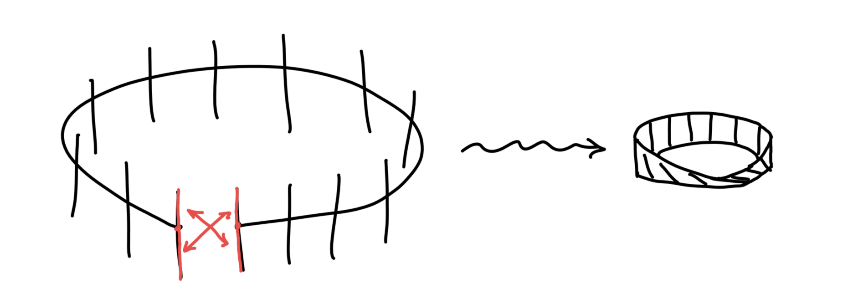
\includegraphics[scale=0.4]{chern_mobius1}
\end{center}

\begin{exercise}
    Check that this defines a vector bundle, by seeing that on an actual open
    cover of $S^1$ we have local trivializations and transition maps, as in the
    following figure.
    \begin{center}
        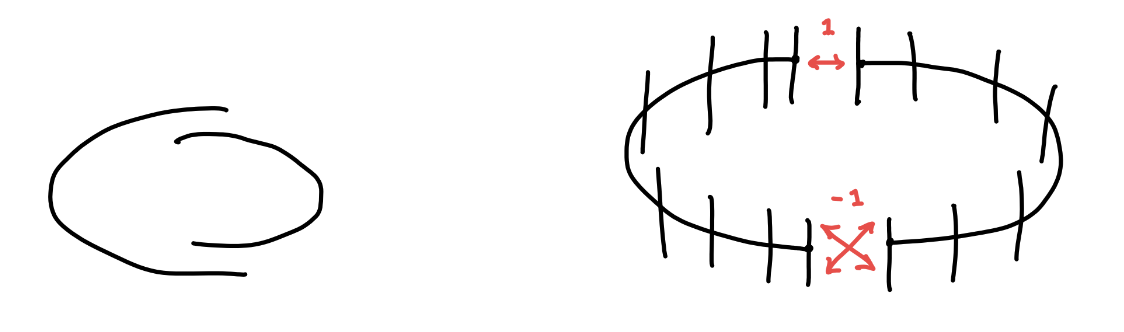
\includegraphics[scale=0.3]{chern_mobius2}
    \end{center}
\end{exercise}

\begin{proof}[Solution]
    With the indicated open cover $S^1=U\cup V$ the intersection $U\cap V$ is a
    disjoint union of two intervals. We glue by $\id$ on one interval and $-\id$
    on the other. This is a locally constant association $U\cap V\to\GL(1,\C)$,
    which is hence continuous.
\end{proof}

\begin{exercise}
    If instead of one twist we include two twists, show that the resulting
    bundle is trivial. Further, show that it can be untwisted to the standard
    band if embedded in $\R^4$.
\end{exercise}

\begin{proof}[Solution]
    If we take two trivializations, where the two twists are contained in one of
    them, then on the two components of the overlap we glue by $\id$ and
    $-(-\id)=\id$, so the trivializations glue to a global trivialization. In
    fact triviality is a consequence of the second part. For the second part,
    note that if we replace one twist of the double-twisted band by the reverse
    oriented twist, then the band can be untwisted to the standard band inside
    $\R^3$:
    \begin{center}
        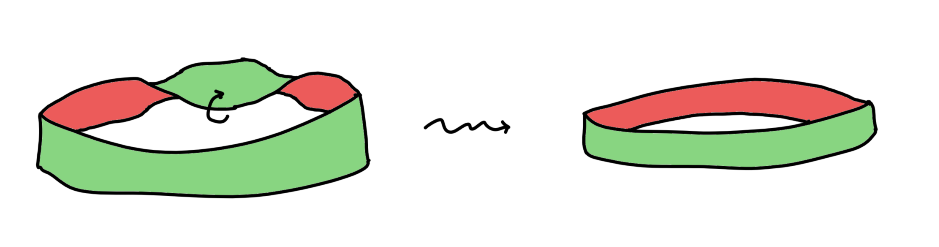
\includegraphics[scale=0.3]{chern_isotopy1}
    \end{center}
    Hence it suffices to show that in $\R^4$ a twist can be reversed. Given a
    twist embedded in $\R^3\times\{0\}\subseteq\R^4$ as pictured below, we can
    achieve this by:
    \begin{itemize}
        \item Perform a straight line isotopy so that the 4th coordinate $x_4$
            is equal to the 2nd coordinate $x_2$.
        \item Perform a straight line isotopy to replace $x_2$ by $-x_2$. This
            leads to no self-intersections since the original coordinates
            can be recovered as $(x_1,x_4,x_3)$.
        \item Perform a straight line isotopy returning $x_4$ to zero. This
            leads to no self-intersections since the original coordinates can
            be recovered as $(x_1,-x_2,x_3)$.
    \end{itemize}
    \begin{center}
        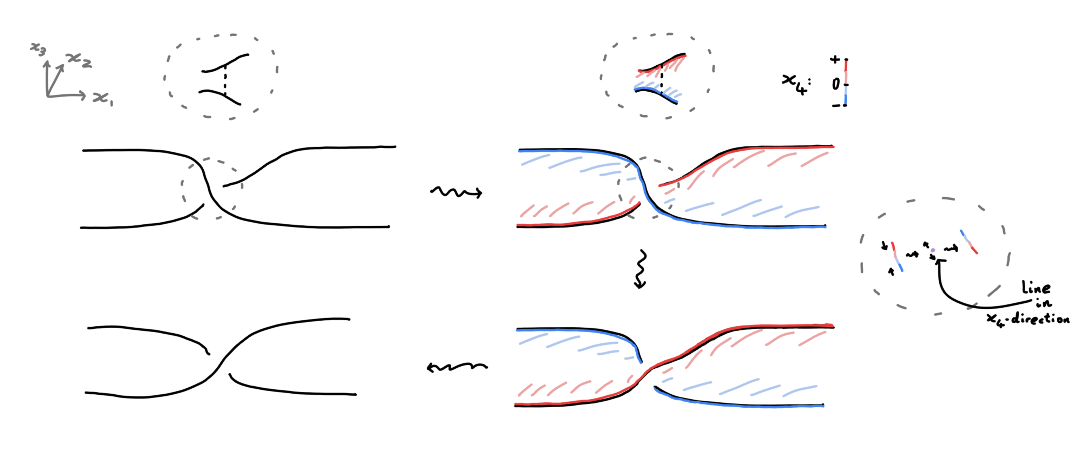
\includegraphics[scale=0.5]{chern_isotopy2}
    \end{center}
\end{proof}

Now we may think of $E$ as $\coprod_U(U\times\C^r)/\sim$, where we glue by the
transition functions $g_{UV}$; for $x\in U\cap V$ we identify
\begin{equation*}
    V\times\C^r\ni(x,e) \sim (x,g_{UV}(x)e)\in U\times\C^r.
\end{equation*}

\begin{exercise}
    Check that this defines an equivalence relation, and that the quotient is
    $E$.
\end{exercise}

\begin{proof}[Solution]
    It is an equivalence relation:
    \begin{itemize}
        \item Reflexive: $(x,e)\sim(x,g_{UU}(x)e)=(x,e)$ as
            $g_{UU}(x)=\id$.
        \item Symmetric: $(x,g_{UV}(x)e)\sim(x,g_{VU}(x)g_{UV}(x)e)=(x,e)$ as
            $g_{VU}(x)\circ g_{UV}(x)=\id$.
        \item Transitive: $(x,e)\sim(x,g_{WV}(x)e)=(x,g_{WU}(x)g_{UV}(x)e)$ as
            $g_{WV}=g_{WU}\circ g_{UV}$.
    \end{itemize}
    We then have a natural map $\coprod_U(U\times\C^r)/\sim\to E$ by the
    universal property of the quotient, which is a homeomorphism over each $U$,
    and a bijection, and therefore a global homeomorphism.
\end{proof}

\begin{exercise}
    Show that the fibres of $\pi$ are naturally vector spaces: if $x_1=(x,e_1)$
    and $x_2=(x,e_2)$ are points of the same fibre $E_x=\pi^{-1}(x)$ and
    $\alpha,\beta\in\C$ we can define $\alpha x_1+\beta x_2\in E_x$ such that...
\end{exercise}

\begin{proof}[Solution]
    In a local trivialization we can take these vector space operations to be
    the natural ones on $\C^r$ under the canonical identification
    $\{x\}\times\C^r\cong\C^r$. This is independent of the choice of local
    trivialization since the vector space operations are preserved by the
    transition maps in $\GL(r,\C)$.
\end{proof}

\begin{exercise}
    Define smooth vector bundles over a smooth manifold, algebraic vector
    bundles over algebraic varieties, real vector bundles, e.t.c.
\end{exercise}

\begin{proof}[Solution]
    For a smooth vector bundle we require the map $U\cap V\to\GL(r,\C)$ to be
    smooth. For an algebraic vector bundle we take local trivializations of the
    form $\pi^{-1}(U)\cong U\times\A^r$, and require $U\cap V\to\GL(r,\C)$ to be
    a regular morphism. For real vector bundles we replace $\C$ by $\R$.
\end{proof}

\paragraph{Sections.} A section of $\pi:E\to X$ is a continuous map $s:X\to E$
such that $\pi\circ s=\id_X$. They form a vector space $\Gamma(E)$ by the
fibre-wise vector space operations.

\begin{exercise}
    A trivialization of the bundle, i.e. an isomorphism
    \begin{equation*}
        \begin{tikzcd}
            &E \ar[d,"\pi"] \ar[r,"\sim"]
                &X\times\C^r \ar[d,"{(x,v)\mapsto x}"] \\
            &X \ar[r,equals] &X
        \end{tikzcd}
    \end{equation*}
    is the same thing as a choice of $r$ sections $s_1,\ldots,s_r$ which form a
    basis at every point, i.e. $s_1(x),\ldots,s_r(x)$ is a basis of $E_x$ for
    every $x\in X$. Hence a trivialization of a line bundle is the same thing as
    a nowhere-vanishing section.
\end{exercise}

\begin{proof}[Solution]
    On a trivial vector bundle $X\times\C^r$ we have a canonical choice of $r$
    sections forming a basis of each fibre given by the basis vectors in $\C^r$;
    every fibre is canonically identified. We can then transport this along the
    isomorphism $E\cong X\times\C^r$ to get such sections for $E$. Conversely,
    given such sections for $E$ we can define an isomorphism
    $E\cong X\times\C^r$ by taking coordinates in $\C^r$ using the basis on each
    fibre.
\end{proof}

\paragraph{Homotopy invariance.} We have
\begin{itemize}
    \item \textbf{Fact 1:} Homotopic bundles are isomorphic. Given
        $E\to X\times[0,1]$, writing $E_t=E|_{X\times\{t\}}$ we have
        $E_0\cong E_1$.

    \item \textbf{Fact 2:} Bundles on contractible spaces $X$ are trivial. If
        $X\simeq\{*\}$ then any bundle $E\to X$ is isomorphic to $X\times\C^r$.
\end{itemize}
For proofs using the Tietze extension theorem see Atiyah's \emph{$K$-Theory}.

So given a rank $r$ bundle $E\to S^n$, we know that restricted to either
hemisphere it is trivial,
\begin{equation*}
    S^n = B^n_1\cup B^n_2, \qquad E|_{B^n_i}\cong B^n_i\times\C^r.
\end{equation*}
These restrictions are glued over the boundary $\partial B^n_i\cong S^{n-1}$ by
a map $S^{n-1}\to\GL(r,\C)$. (Strictly speaking we should take slightly larger
open hemispheres, intersecting in an open annulus which contracts to this
boundary.)

\paragraph{Clutching construction.}

So rank $r$ complex bundles on $S^n$ are in 1-1 correspondence with homotopy
classes of maps $S^{n-1}\to\GL(r,\C)$, i.e. with
\begin{equation*}
    \pi_{n-1}(\GL(r,\C)).
\end{equation*}
E.g. real version with $r=1$ gives
\begin{equation*}
    \{\text{line bundles on $S^1$}\}
        \leftrightarrow \pi_0(\GL(1,\R))
        = \pi_0(\R^\times)
        = \Z/2.
\end{equation*}
(Note that this isn't exactly an example of the previous discussion, since here
the group is disconnected.) This mod 2 integer is the Stiefel--Whitney class of
the bundle.

\paragraph{First Chern class.}
E.g. complex version with $r=1$ gives
\begin{equation*}
    \{\text{line bundles on $S^2$}\}
        \leftrightarrow \pi_1(\GL(1,\C)) = \pi_1(\C^\times) = \Z.
\end{equation*}
This integer classifying the bundle is called its \emph{first Chern class},
$c_1$. For an algebraic version, write
\begin{equation*}
    S^2 \cong \P^1 = \C_x\cup_{\C^\times}\C_y
\end{equation*}
glued over $\C^\times=\{x\ne0\}=\{y\ne0\}$ by $x=\frac{1}{y}$. Then glue trivial
line bundles $\C_x\times\C$ and $\C_y\times\C$ by
\begin{equation*}
    (x,t) \mapsto \biggl(\frac{1}{x},x^{-n}t\biggr) = (y,y^nt).
\end{equation*}
We call the resulting line bundle $\O(n)$ with $c_1=n$.

\paragraph{Tautological bundle.}
When $n=-1$ we get the \emph{tautological bundle} $\O(-1)\to\P^1$. Over $\R$
this is the M\"obius bundle on $\RP^1\cong S^1$:
\begin{center}
    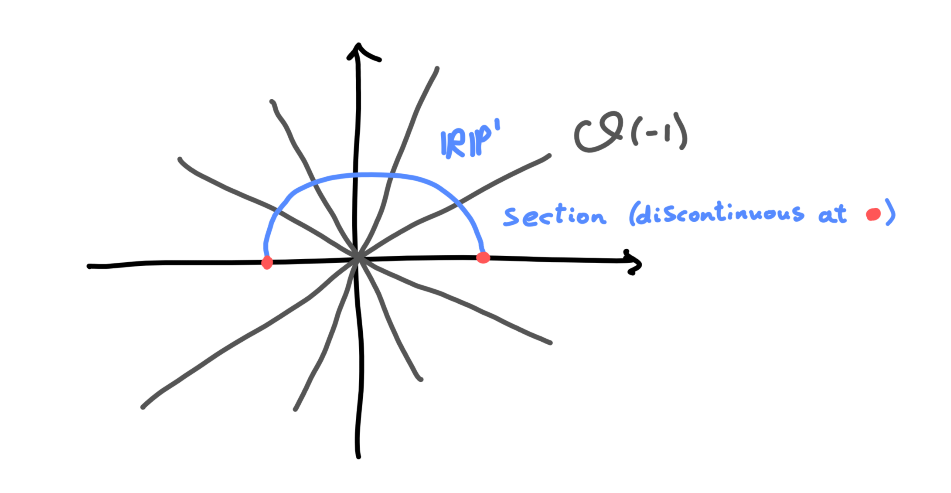
\includegraphics[scale=0.5]{chern_taut1}
\end{center}

\paragraph{Tautological bundle over $\C$.}
Over $\C$ we also see that $\O(-1)$ (defined as above with transition
function $\frac{1}{x}$) is the tautological bundle $\O(-1)$ over $\P^1$.
\begin{center}
    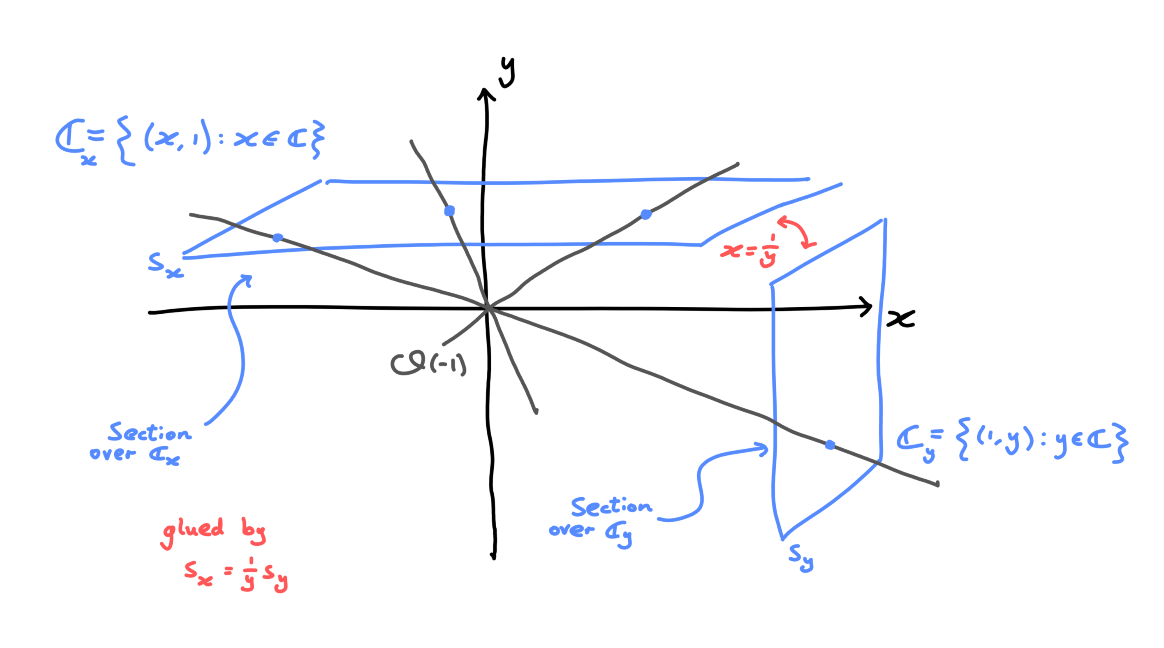
\includegraphics[scale=0.5]{chern_taut2}
\end{center}
We can check that the section $s_x$ when viewed over $\C_y$ does not extend
continuously over the origin, so it doesn't give a trivialization of the whole
bundle.

\paragraph{Zeros of sections.}
The $\O(n)$ line bundle over $\P^1$ was defined with transition function
$x^{-n}$, gluing the section 1 over $\C_x$ to $x^{-n}=y^n$ over $\C_y$. This
therefore defines a \emph{global} holomorphic section of $\O(n)$ when
$n\ge0$, with a degree $n$ zero at $y=0$. (If $n<0$ we get a meromorphic section
with a degree $n$ pole at $y=0$.)

Similarly $p(x)$ over $\C_x$ is glued to $y^np(y^{-1})$ over $\C_y$, so if
$\deg p=n$ we get another algebraic/regular section over $\P^1$. (This gives all
the sections since $\Gamma(\O(n))=\Sym^n(\C^2)^*$.) Again these all have $n$
zeros.

\begin{exercise}
    When $n<0$ we get a meromorphic section with $n$ poles. Instead glue 1 to an
    anti-holomorphic function across the circle $|x|=1$ to give a
    (non-holomorphic) section with $n$ zeros.
\end{exercise}

\begin{proof}[Solution]
    We can glue $1/z^n$ outside the unit circle to $\conj z^n$ inside the unit
    circle, since they agree on the boundary. (If $|z|=1$ then $1/z=\conj z$.)
\end{proof}

\paragraph{Intersection with the zero section.}
Indeed $c_1=n$ is the number of zeros (counted with orientation and
multiplicity) of \emph{any} section of $\O(n)$. In other words, $c_1(L)$ is
the \emph{intersection of the zero section of $L$} with itself (or equivalently
with the graph of any other section).
\begin{center}
    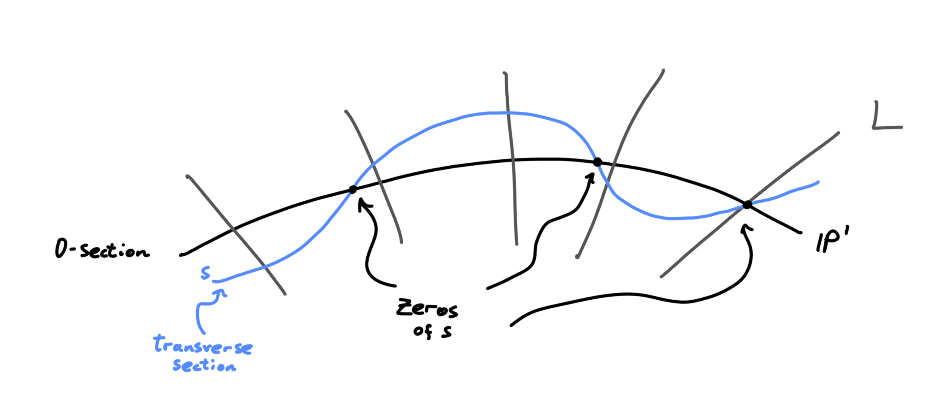
\includegraphics[scale=0.6]{chern_section}
\end{center}

\paragraph{Clutching construction on arbitrary Riemann surfaces.}
Again line bundles are trivial bundles glued across circles / annuli.
\begin{center}
    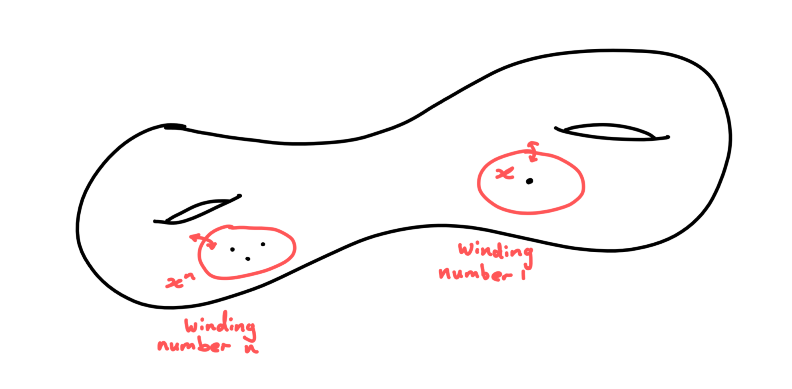
\includegraphics[scale=0.6]{chern_clutch}
\end{center}
\begin{align*}
    c_1(L)
        &= \text{total winding number of transition functions} \\
        &= \text{number of zeros of a section}.
\end{align*}
(So under the line bundle $\leftrightarrow$ divisor correspondence,
$c_1(\O(D))=\deg D$.)

\paragraph{First Chern class on manifolds.}
More generally for any complex line bundle $L$ on a manifold $M$ we define
\begin{equation*}
    c_1(L) = [s^{-1}(0)]\in H_{\dim X-2}(X)
\end{equation*}
where $s$ is any section \emph{transverse to the zero section}. (If $s'$ is
another choice then we have a homotopy $s_t=(1-t)s+ts'$ so that $s_t^{-1}(0)$ is
a chain interpolating from $s$ to $s'$.)

In fact we can define $c_1(L)$ to be the Poincar\'e dual of $[s^{-1}(0)]$, as
this cohomology class will generalize to arbitrary topological spaces $X$. For
general $X$ we can understand $c_1(L)\in H^2(X)$ by evaluating it on
$[\Sigma]\in H_2(X)$ for Riemann surfaces $\Sigma\hookrightarrow X$, by
\begin{equation*}
    \langle c_1(L),[\Sigma]\rangle = c_1(L|_\Sigma).
\end{equation*}

\paragraph{Higher Chern classes on manifolds.}
For any rank $r$ complex vector bundle $E\to X$ pick a transverse
$C^\infty$-section $s$ and define the \emph{Euler class} or top Chern class
\begin{equation*}
    e(E) = c_r(E) = [s^{-1}(0)] \in H_{\dim X-2r}(X) \cong H^{2r}(X).
\end{equation*}
Analogously define
\begin{equation*}
    c_k(E) \in H^{2k}(X)
\end{equation*}
to be Poincar\'e dual to the locus where $r-k+1$ generic sections fail to be
linearly independent:
\begin{equation*}
    [(s_1\wedge\cdots\wedge s_{r-k+1})^{-1}(0)] \in H_{\dim X-2}(X).
\end{equation*}
So $c_r(E)=e(E)$ while $c_1(E)=c_1(\Lambda^rE)$ and $c_i(E)=0$ for $i>r$.
(When $k\ne1,r$ note that $c_k(E)\ne e(\Lambda^{r-k+1}E)$---this has the wrong
degree, and $s_1\wedge\cdots\wedge s_{r-k+1}$ is \emph{not} a generic section of
$\Lambda^{r-k+1}E$.)

\paragraph{Whitney sum formula.}
Given two generic sections $s_1\in\Gamma(E_1)$, $s_2\in\Gamma(E_2)$ where $E_i$
has rank $r_i$, we get a section $s_1\oplus s_2\in\Gamma(E_1\oplus E_2)$, with
\begin{equation*}
    e(E_1\oplus E_2)
        = [(s_1\oplus s_2)^{-1}(0)]
        = [s_1^{-1}(0)\cap s_2^{-1}(0)]
        = e(E_1)\cup e(E_2) \in H^{2r_1+2r_2}.
\end{equation*}
In particular, for line bundles
$c_2(L_1\oplus L_2)=c_1(L_1)\cup c_1(L_2)$ and
\begin{align*}
    c_1(L_1\oplus L_2)
        &= c_1(\Lambda^2(L_1\oplus L_2)) \\
        &= c_1(L_1\otimes L_2) \\
        &= [(s_1\otimes s_2)^{-1}(0)] \\
        &= [s_1^{-1}(0)\cup s_2^{-1}(0)] \\
        &= c_1(L_1) + c_1(L_2).
\end{align*}
We can write this as $c(L_1\oplus L_2)=c(L_1)\cup c(L_2)$ where the
\emph{total Chern class} is defined as
\begin{equation*}
    c(E)=1+c_1(E)+c_2(E)+\cdots\in H^*(X).
\end{equation*}
More generally, for bundles $E,F$ of rank $r,s$ use the decomposition
\begin{equation*}
    \Lambda^k(E\oplus F) = \bigoplus_{i=0}^k\Lambda^i(E)\otimes\Lambda^{k-i}(F)
\end{equation*}
and generic sections $e_1,\ldots,e_k\in\Gamma(E)$ and
$f_1,\ldots,f_k\in\Gamma(F)$ to compute
\begin{align*}
    \bigl[\bigl(&(e_1\wedge\cdots\wedge e_k)
        \oplus(e_1\wedge\cdots\wedge e_{k-1}\otimes f_k)
        \oplus\cdots \\
           &\qquad\oplus(e_1\otimes f_2\wedge\cdots\wedge f_k)
           \oplus(f_1\wedge\cdots\wedge f_k)
       \bigr)^{-1}(0)\bigr].
\end{align*}

\begin{exercise}
    Work it out and take Poincar\'e duals to give
    \begin{equation*}
        c_{r+s-k+1}(E\oplus F)
            = c_r(E)c_{s-k+1}(F) + \cdots + c_{r-k+1}(E)c_s(F).
    \end{equation*}
    Deduce the \emph{Whitney sum formula} $c(E\oplus F)=c(E)c(F)$.
\end{exercise}

\begin{proof}[Solution]
    For the given definition of $c_{r+s-k+1}(E\oplus F)$, we take generic
    sections $e_1\oplus f_1,\ldots,e_k\oplus f_k$ of $E\oplus F$, and consider
    their wedge product. Under the decomposition
    $\Lambda^k(E\oplus F)=\bigoplus_{i=0}^k\Lambda^i(E)\otimes\Lambda^{k-i}(F)$
    this is given by
    \begin{align*}
        (e_1\oplus f_1)\wedge\cdots\wedge(e_k\oplus f_k)
            &= (e_1\wedge\cdots\wedge e_k)
                \oplus(e_1\wedge\cdots e_{k-1}\otimes f_k)
                \oplus\cdots \\
            &\qquad\oplus(e_1\otimes f_2\wedge\cdots\wedge f_k)
                \oplus(f_1\wedge\cdots\wedge f_k),
    \end{align*}
    and $c_{r+s-k+1}(E\oplus F)$ is represented by the Poincar\'e dual of the
    vanishing locus of this section.

    \textbf{Set-theoretical Claim:} Given a set $S$ with chains of subsets
    \begin{equation*}
        A_0\subseteq A_1\subseteq\cdots\subseteq A_k=S
        \quad\text{and}\quad
        S=B_0\supseteq B_1\supseteq\cdots\supseteq B_k,
    \end{equation*}
    we have
    \begin{equation*}
        \bigcap_{i=0}^k(A_i\cup B_i)
            = \bigcup_{j=1}^k(A_j\cap B_{j-1}).
    \end{equation*}

    Applying this to the subsets $A_i=(e_1\wedge\cdots\wedge e_i)^{-1}(0)$,
    $B_i=(f_{i+1}\wedge\cdots\wedge f_k)^{-1}(0)$ of $X$, we get
    \begin{align*}
        &\bigl[(e_1\wedge\cdots\wedge e_k)^{-1}(0)
            \cap(e_1\wedge\cdots\wedge e_{k-1}\otimes f_k)^{-1}(0)
            \cap\cdots \\
        &\qquad\qquad\cap(e_1\otimes f_2\wedge\cdots\wedge f_k)^{-1}(0)
            \cap(f_1\wedge\cdots\wedge f_k)^{-1}(0)
        \bigr] \\
        &\qquad=\biggl[\bigcap_{i=0}^k
            \bigl((e_1\wedge\cdots\wedge e_i)^{-1}(0)
        \cup(f_{i+1}\wedge\cdots\wedge f_k)^{-1}(0)\bigr)\biggr] \\
        &\qquad=\biggl[\bigcup_{j=1}^k
            \bigl((e_1\wedge\cdots\wedge e_j)^{-1}(0)
            \cap(f_j\wedge\cdots\wedge f_k)^{-1}(0)\bigr)\biggr], \\
    \end{align*}
    and hence
    \begin{align*}
        c_{r+s-k+1}(E\oplus F)
            &= \sum_{j=1}^kc_{r-j+1}(E)c_{s-k+j}(F) \\
            &= c_r(E)c_{s-k+1}(F) + \cdots + c_{r-k+1}(E)c_s(F).
    \end{align*}
\end{proof}

\paragraph{Axiomatic approach.}

\begin{fact}
    Knowing (or defining!) $c_1(\O_{\P^n}(1))=[\P^{n-1}]$, the Whitney sum
    formula and functoriality is then enough to completely determine all Chern
    classes on all topological spaces.
\end{fact}

Functoriality: $c(f^*E)=f^*c(E)$.

\begin{exercise}
    Define $f^*E$ and prove this using zero loci of sections when $f:X\to Y$ is
    a map of manifolds.
\end{exercise}

\begin{proof}[Solution]
    Given local trivializations $E|_U\cong U\times\C^r$, we define a local
    trivialization $f^*E|_{f^{-1}(U)}\cong f^{-1}(U)\times\C^r$ by associating
    $(x,v)\in f^{-1}(U)\times\C^r$ with $(f(x),v)\in U\times\C^r$. The
    transition functions are given by the transition functions for $E$ composed
    with $f$, and hence remain continuous, so this defines a vector bundle. Then
    if $s_1,\ldots,s_k$ are generic sections of $E$, we get that
    $f^*s_1,\ldots,f^*s_k$ are generic sections of $f^*E$ since all sections of
    $f^*E$ are pullbacks of sections of $E$. (Assuming $X$ and $Y$ are compact,
    so $f$ is closed.) Moreover the vanishing locus of
    $f^*s_1\wedge\cdots\wedge f^*s_k=f^*(s_1\wedge\cdots\wedge s_k)$ is the
    preimage under $f$ of the vanishing locus of $s_1\wedge\cdots\wedge s_k$.
    Since the cohomology class of the preimage gives the pullback of the
    cohomology class (for suitably general representatives missing critical
    values of $f$) this shows naturality of the Chern class.
\end{proof}

There are two steps to proving this fact:
\begin{itemize}
    \item All rank $r$ bundles on $X$ are pullbacks $f^*Q$ of the
        \emph{universal bundle on the classifying space} $Q\to B\GL(r,\C)$ by a
        map $f:X\to B\GL(r,\C)$. (So we only need to define $c_i$ on one
        classifying space.)

    \item Splitting principle: We may assume $E$ is a direct sum of line bundles
        without loss of generality.
\end{itemize}

\paragraph{Classifying space.}
Any bundle $E$ is a quotient of an infinite rank trivial bundle
$\underline{\Gamma(E)}$ (here $\underline V$ denotes the trivial bundle with
fibre $V$):
\begin{equation*}
    \underline{\Gamma(E)} \xrightarrow{\ev} E\to 0. \tag{$*$}
\end{equation*}
(Or take a sufficiently large subbundle
$\underline\C^N\subseteq\underline\C^\infty=\underline{\Gamma(E)}$, $N\gg0$.)
Therefore it defines a map from $X$ to the Grassmannian
\begin{align*}
    f:X&\to\Gr(\C^\infty,r), \\
    x &\mapsto (*)_x.
\end{align*}
There is a tautological universal quotient bundle $Q\to\Gr(\C^\infty,r)$
\begin{equation*}
    \underline\C^\infty \to Q \to 0 \qquad \text{over $\Gr(\C^\infty,r)$,}
\end{equation*}
and from ($*$) we get that $f$ pulls this back to give $E$; $f^*Q\cong E$. Thus
$\Vect_r(X)=[X,\Gr(\C^\infty,r)]$. We call $\Gr(\C^\infty,r)$ the
\emph{classifying space} $B\GL(r,\C)$. For example, if $r=1$ we have
$B\C^\times=\CP^\infty$, so any line bundle $\L\to X$ is $f^*\O(1)$ for some
(homotopy class of) map $f:X\to\CP^\infty$ (or $f:X\to\CP^N$ for $N\gg0$ if $X$
is finite dimensional). Then
\begin{equation*}
    c_1(\L) = f^*c_1(\O(1)) = f^*h
\end{equation*}
where $h\in H^2(\CP^\infty)$ is the generator (the limit as $N\to\infty$ of the
Poincar\'e duals of $\CP^{N-1}\subseteq\CP^N$, or the standard K\"ahler form).

\paragraph{Splitting principle.}
Given $E\to X$ (e.g. $Q\to\Gr(\C^\infty,r)$) there is a space dominating $X$ on
which $E$ splits as a sum of line bundles:
\begin{equation*}
    \pi:Y\to X \quad \text{such that} \quad \pi^*E=\L_1\oplus\cdots\oplus\L_r,
\end{equation*}
with fibres $Y_x=\pi^{-1}(x)$ given by the flag manifolds
\begin{equation*}
    Y_x = \{\text{linearly independent complex line bundles
        $L_1,\ldots,L_r\subseteq E_x$}\}.
\end{equation*}
There are universal / tautological bundles $\L_i$ on $Y$, and it is then
tautological that $\pi^*E\cong\oplus_{i=1}^r\L_i$.

\textbf{Fact:} $\pi^*:H^*(X)\to H^*(Y)$ is an injection, so pulling back $c(E)$
loses no information, and
\begin{equation*}
    \pi^*c(E) = c(\pi^*E) = c(\L_1\oplus\cdots\oplus\L_r)
        = c(\L_1)\cdots c(\L_r).
\end{equation*}
Hence for $E\to X$ we get a diagram
\begin{equation*}
    \begin{tikzcd}
        &Y \ar[r,"f"] \ar[d,"\pi"] &B(\C^\times)^r = (\CP^\infty)^r \\
        &X
    \end{tikzcd}
\end{equation*}
such that $\pi^*:H^*(X)\to H^*(Y)$ is an injection, and $c(E)\in H^*(X)$ is the
unique class such that
\begin{equation*}
    \pi^*c(E) = f^*[(1+h_1)\cdots(1+h_r)].
\end{equation*}
So the splitting principle, the Whitney sum formula, and $c_1(\O(1))=h$
determine all Chern classes uniquely. (Existence takes a little bit more work,
e.g. computing $H^*(\Gr(\C^\infty,r))$.)

\begin{exercise}
    Prove the following corollary: If $E$ has rank $r$, then $c_i(E)=0$ for
    $i>r$.
\end{exercise}

\begin{proof}[Solution]
    From above we have
    \begin{equation*}
        \pi^*c(E) = (1+f^*h_1)\cdots(1+f^*h_r)
    \end{equation*}
    where $h_1,\ldots,h_r$ have degree 1, so the RHS has no terms in degree
    $i>r$. Hence $\pi^*c_i(E)=0$, and since $\pi^*$ is injective $c_i(E)=0$.
\end{proof}

\paragraph{Grothendieck's definition.}
On the projective bundle $\pi:\P(E)\to X$ we have the tautological inclusion
\begin{equation*}
    \O_{\P(E)}(-1) \hookrightarrow \pi^*E.
\end{equation*}
Since the quotient bundle is of rank $r-1$,
\begin{equation*}
    c_r(\pi^*E/\O_{\P(E)}(-1)) = 0.
\end{equation*}
By the Whitney sum formula, this is the degree $r$ part of
\begin{equation*}
    \pi^*c(E)/c(\O_{\P(E)}(-1)) = \pi^*c(E)/(1-h),
\end{equation*}
where $h=c_1(\O_{\P(E)}(-1))$. Thus
\begin{equation*}
    h^r + \pi^*c_1(E)h^{r-1} + \cdots + \pi^*c_{r-1}(E)h + \pi^*c_r(E) = 0.
        \tag{$*$}
\end{equation*}
\textbf{Fact:} $H^*(\P(E))
=H^*(X)\oplus H^*(X)h\oplus\cdots\oplus H^*(X)h^{r-1}$, so $h^r$ can be uniquely
written as a linear combination of $1,h,\ldots,h^{r-1}$ and we can define
$c_i(E)$ via ($*$).

\paragraph{Chern--Weil for line bundles.}
If $X$ is a manifold we can pick a connection $A$ on $\L\to X$. Its curvature
$F_A$ is a closed 2-form; $dF_A=0$. Changing $a\mapsto A+a$ gives
$F_A\mapsto F_A+da$, so $[F_A]\in H^2(X;\R)$ is independent of $A$. In fact it
is given by
\begin{equation*}
    \frac{[F_A]}{2\pi i} = [c_1(\L)] \in H^2(X;\Z)/\text{torsion}.
\end{equation*}
Let's prove this for $X$ a Riemann surface and $\L$ described by the clutching
construction. Write $X=U\cup_{S^1}D^2$ where $D^2$ is a disc and $S^1$ is an
annulus thickening its boundary. Write $\L$ as
$\underline\C_U\cup_\phi\underline\C_{D^2}$ for a transition function
$\phi:S^1\to\C^\times$ of winding number $n=c_1(\L)$. Put the trivial connection
$d$ on $\underline\C_U$. In the trivialization $\underline\C_D$ restricted to
the annulus this is the connection
\begin{equation*}
    d+\phi^{-1}d\phi
\end{equation*}
since this annhilates $\phi$ (which is glued to 1 on $U$). Extend this to any
connection $d+a$ over $D^2$ and compute
\begin{align*}
    \int_XF_A = \int_{D^2}F_A = \int_{D^2}da = \int_{S^1}da
              = \int_{S^1}\frac{d\phi}{\phi} = \int_{S^1}d\log\phi
              = 2\pi in.
\end{align*}

\paragraph{Chern--Weil theory.}
Suppose $X$ is a manifold with a rank $r$ bundle $E\to X$ and a connection $A$
on $E$. Form
\begin{equation*}
    p\biggl(\frac{F_A}{2\pi i}\biggr) \in H^{2k}(X;\R)
\end{equation*}
for any ad-invariant ($p(N^{-1}MN)=p(M)$) polynomial function $p$ of
$\End(\C^r)$. For example $p$ could be $\tr$ (giving $c_1(E)$), or $\det$
(giving $c_r(E)$), or any other symmetric polynomial in the eigenvalues. (In
fact $H^*(B\GL(r,\C))=\text{Ad-invariant polynomials}$.) If $p$ is integral, the
result is an integral characteristic class.

\begin{exercise}
    Show that $p(F_A)$ is closed, and changes by an exact form under
    $A\mapsto A+a$. % TODO
\end{exercise}

\begin{theorem}
    We have $c(E)=\det(\id+\frac{F_A}{2\pi i})$ in $H^*(X)/\text{torsion}$, i.e.
    \begin{equation*}
        1 + c_1(E) + c_2(E) + \cdots
            = 1 + \frac{\tr F_A}{2\pi i} - \frac{\tr(F_A\wedge F_A)}{4\pi^2}
                + \cdots.
    \end{equation*}
\end{theorem}

\paragraph{Tangent bundle to projective space.}
Let $V=\C^{n+1}$ so that $\P(V)=\P^n$. Then
\begin{equation*}
    T_{\P^n} = \O(-1)^*\otimes\underline V/\O(-1).
\end{equation*}
\begin{proof}[Sketch]
    A point of $\P(V)$ is a complex line $L\le V$. Pick any complement to write
    $V=L\oplus V/L$. Then nearby lines in $V$ are graphs of linear maps
    $L\to V/L$. So the tangent space is $L^*\otimes V/L$.
\end{proof}
\begin{center}
    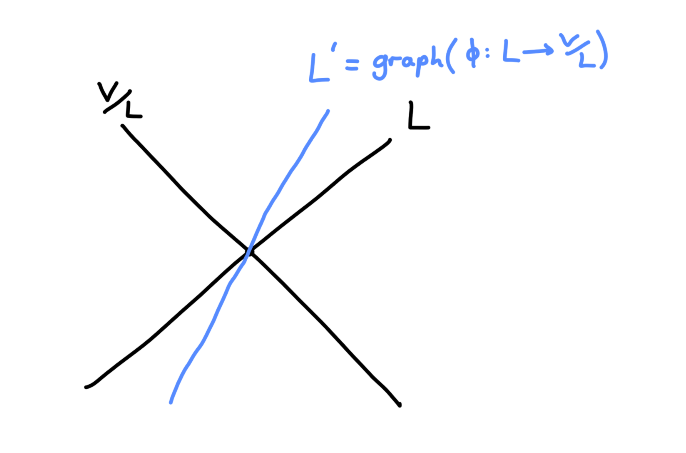
\includegraphics[scale=0.4]{chern_tangent}
\end{center}

\paragraph{Chern classes of projective space.}
Applying the Whitney sum formula to $T_{\P^n}=\underline V(1)/\O(-1)$ gives
\begin{equation*}
    c(T_{\P^n})
        = c(\underline V(1))/c(\O(-1))
        = c(\O(1)^{\oplus(n+1)})
        = (1+h)^{n+1},
\end{equation*}
where $h=c_1(\O(1))$ is the hyperplane class Poincar\'e dual to
$\P^{n-1}\subseteq\P^n$. (So for example $c_n(T_{\P^n})=(n+1)h^n$, and
integrating gives $e(\P^n)=n+1$.)

\paragraph{Hypersurfaces in projective space.}
\begin{exercise}
    ``Adjunction'': If $s\in\Gamma(E)$ is transverse to the zero section, show
    its zero locus $Z=s^{-1}(0)$ has normal bundle $N_{Z/X}=E|_Z.$
    \begin{center}
        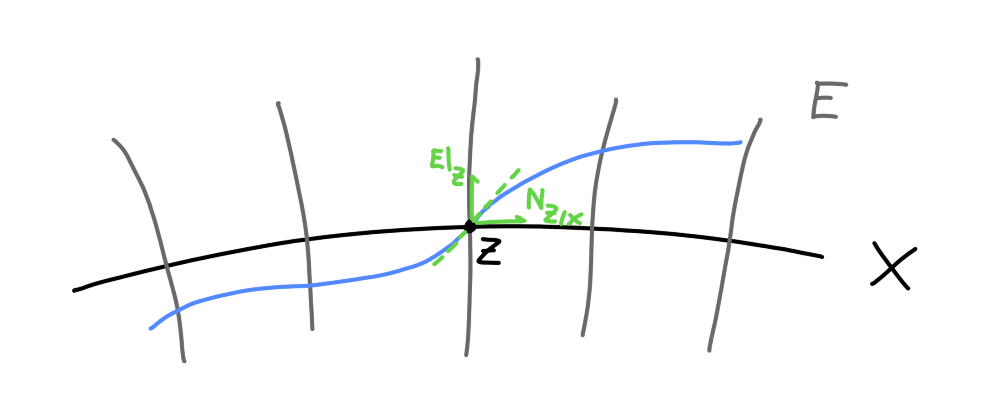
\includegraphics[scale=0.5]{chern_normal}
    \end{center}
\end{exercise}

\begin{proof}[Solution]
    Note that $TE=\pi^*(TX\oplus E)$, and so the derivative of $s$ gives a map
    \begin{equation*}
        TX\to s^*TE = s^*\pi^*(TX\oplus E) = TX\oplus E
    \end{equation*}
    whose projection to $TX$ is the identity. The condition of being transverse
    to the zero section means that the projection to $E$ is non-zero over $Z$.
    Furthermore, note that $TX|_Z=TZ\oplus N_{Z/X}$, and the derivative of $s$
    vanishes on $TZ$ since $s|_Z=0$. Therefore the composite
    \begin{equation*}
        TZ\oplus N_{Z/X} = TX|_Z \to TX|_Z\oplus E|_Z \to E|_Z
    \end{equation*}
    vanishes on $TZ$, but is non-zero and hence induces an isomorphism
    $N_{Z/X}\to E|_Z$ of line bundles.
\end{proof}

\begin{exercise}
    Hence work out the total Chern class $c(T_{X_d})$ of a degree $d$
    hypersurface $X_d\subseteq\P^n$ (the zero locus of a section of $\O(d)$).
    Apply to $n=3$, $d=4$ to find $c_1(T_S)$ and $e(S)$ for $S$ a ``K3
    surface''.
\end{exercise}

\begin{proof}[Solution]
    Let $i:X_d\hookrightarrow\P^n$ denote the inclusion. Note that
    $i^*T_{\P^n}=T_{X_d}\oplus N_{X_d/\P^n}$, so by the Whitney sum
    formula
    \begin{equation*}
        c(T_{X_d}) = c(i^*T_{\P^n})/c(N_{X_d/\P^n}).
    \end{equation*}
    But from naturality of the Chern class, and the above computation of
    $c(T_{\P^n})$, we have
    \begin{equation*}
        c(i^*T_{\P^n}) = i^*(1+h)^{n+1} = (1+\omega)^{n+1},
    \end{equation*}
    where $\omega=i^*h$. Moreover the previous exercise gives
    $N_{X_d/\P^n}\cong i^*\O(d)$, so by naturality and the Whitney sum formula
    \begin{equation*}
        c(N_{X_d/\P^n})
            = c(i^*\O(d))
            = i^*(1+c_1(\O(1)^{\otimes d}))
            = (1+d\cdot\omega).
    \end{equation*}
    Hence
    \begin{equation*}
        c(T_{X_d}) = (1+\omega)^{n+1}/(1+d\cdot\omega).
    \end{equation*}
    When $n=3$ and $d=4$ we have $\omega^3=0$, and
    \begin{align*}
        c(T_S)
            &= (1+\omega)^4/(1+4\omega) \\
            &= (1+4\omega+6\omega^2)(1-4\omega+16\omega^2) \\
            &= 1+6\omega^2.
    \end{align*}
    Hence $c_1(T_S)=0$ and $e(T_S)=6\omega^2$.
\end{proof}

\begin{exercise}
    Compute $c_i(\End(E))$ in terms of $c_i(E)$ for $E$ a rank 2 bundle. (Hint:
    Splitting principle.) Why did you find $c_1=0=c_3=c_4$?
\end{exercise}

\begin{proof}[Solution]
    First assume $E=L_1\oplus L_2$ is a sum of line bundles. Then
    $\End(E)=\bigoplus_{i,j}L_i^*\otimes L_j$, so by the Whitney sum formula
    \begin{align*}
        c(\End(E))
            &= \prod_{i,j}c(L_i^*\otimes L_j) \\
            &= \prod_{i,j}(1 + c_1(L_j) - c_1(L_i)) \\
            &= 1 + 2c_1(L_1)c_1(L_2) - c_1(L_1)^2 - c_1(L_2)^2 \\
            &= 1 + 4c_2(E) - c_1(E)^2.
    \end{align*}
    This then holds in general by the splitting principle and the naturality of
    the Chern class. We get that the only non-vanishing Chern class of $\End(E)$
    is $c_2(\End(E))=4c_2(E)-c_1(E)^2$.
\end{proof}

\begin{exercise}
    ~
    \begin{enumerate}[label=(\arabic*)]
        \item Compute $c_4(\Sym^3(E))$ in terms of $c_i(E)$ for $E$ a rank 2
            bundle. (Hint: Splitting principle.)

        \item The Grassmannian $\Gr(2,\C^4)$ of 2-planes in $\C^4$ has a
            universal subbundle $\U\hookrightarrow\underline\C^4$. Describe a
            cycle Poincar\'e dual to $c_2(\U^*)$. (Hint: Use
            $(\underline\C^4)\twoheadrightarrow\U^*$ to pick a section of
            $\U^*$.)

        \item Describe a cycle Poincar\'e dual to $c_1(\U^*)$. (Hint: Pick two
            sections of $\U^*$ and see where they're linearly dependent.)
    \end{enumerate}
\end{exercise}

\begin{proof}[Solution]
    \begin{enumerate}[label=(\arabic*)]
        \item By the splitting principle and naturality we may assume
            $E=L_1\oplus L_2$ is a sum of line bundles. Then
            \begin{equation*}
                \Sym^3(E) = \bigoplus_{k=0}^3
                    \bigl(L_1^{\otimes k}\otimes L_2^{\otimes(3-k)}\bigr),
            \end{equation*}
            so by the Whitney sum formula
            \begin{equation*}
                c(\Sym^3(E))
                    = \prod_{k=0}^3\bigl(1 + kc_1(L_1) + (3-k)c_1(L_2)\bigr).
            \end{equation*}
            Writing $\gamma_i=c_1(L_i)$, we then have
            \begin{align*}
                c_4(\Sym^3(E))
                    &= 9\gamma_1\gamma_2
                        (\gamma_1+2\gamma_2)(2\gamma_1+\gamma_2) \\
                    &= 9\gamma_1\gamma_2
                        \bigl(2(\gamma_1+\gamma_2)^2 + \gamma_1\gamma_2\bigr) \\
                    &= 18c_2(E)c_1(E)^2 + 9c_2(E)^2.
            \end{align*}

        \item The class $c_2(\U^*)$ is Poincar\'e dual to the vanishing locus of
            a generic section of $\U^*$. Using the inner product on $\C^4$ we
            have a decomposition $\C^4=\U\oplus\U^*$, and then a generic section
            of $\U^*$ is the image $\langle v,-\rangle$ of a generic section $v$
            of $\underline\C^4$. The vanishing locus of this section is the set
            of planes perpendicular to a continuously varying vector, which if
            we take a constant vector gives $\Gr(2,\C^3)\subseteq\Gr(2,\C^4)$.

        \item Taking two sections $\langle v_1,-\rangle$ and
            $\langle v_2,-\rangle$ of $\U^*$, they are linearly dependent at the
            planes whose orthogonal complements intersect the span
            $\langle v_1,v_2\rangle$. Swapping with orthogonal complements we
            then see that $c_1(\U^*)$ is Poincar\'e dual to the cycle given by
            those planes intersecting $\C^2\subseteq\C^4$ in $\Gr(2,\C^4)$.
    \end{enumerate}
\end{proof}

\begin{exercise}
    Using (1,2,3) above, show that $\int_{\Gr(2,\C^4)}c_4(\Sym^3\U^*)=27$.
\end{exercise}

\begin{proof}[Solution]
    Note that the self-intersection of the cycle Poincar\'e dual to $c_2(\U^*)$
    from (2) is the intersection $\Gr(2,V)\cap\Gr(2,W)=\Gr(2,V\cap W)$ for
    generic 3-dimensional subspaces $V,W\subseteq\C^4$. Now generically
    $\dim(V\cap W)=2$, so this is a single point. Hence $c_2(\U^*)^2$ is
    Poincar\'e dual to the cycle represented by a point, i.e. it is the standard
    generator $\omega\in H^4(\Gr(2,\C^4))$. Also, the self-intersection of the
    cycle Poincar\'e dual to $c_1(\U^*)$ from (3) is represented by the planes
    intersecting two generic copies of $\C^2$ in $\C^4$, which are the sums of
    lines in $\C^2$ with lines in a chosen complement of $\C^2$. Intersecting
    this with the cycle Poincar\'e dual to $c_2(\U^*)$ from (2) gives a point,
    since a generic copy of $\C^3$ intersects both copies of $\C^2$ in a line.
    Hence $c_2(\U^*)c_1(\U^*)^2$ is also $\omega$, and we get
    \begin{equation*}
        \int_{\Gr(2,\C^4)}c_4(\Sym^3\U^*)
            = \int_{\Gr(2,\C^4)}(18\omega+9\omega)
            = 27\int_{\Gr(2,\C^4)}\omega
            = 27
    \end{equation*}
    since the integral of $\omega$ is the intersection number of $\Gr(2,\C^4)$
    with a point, which is 1.
\end{proof}

\begin{exercise}
    Identify $\Gr(2,\C^4)$ with $\{\text{lines $\P^1\subseteq\P^3$}\}$. Let
    $s\in\Gamma(\O_{\P^3}(3))$ cut out a cubic surface $S\subseteq\P^3$. Show
    that $s$ defines a section of $\Sym^3\U^*$ over $\Gr(2,\C^4)$ cutting out
    the lines in $\P^3$ which lie in $S$, of which there are hence 27.
\end{exercise}

\begin{proof}[Solution]
    Pulling back $s$ gives a section of $\O_{\P^1}(3)$ for each line
    $\P^1\subseteq\P^3$. Now $\O_{\P(V)}(d)\cong\Sym^dV^*$, both having bases
    given by monomials, so from this we get a section of $\Sym^3\U^*$ since each
    $\P^1$ corresponds to the projectivization of the associated fibre of $\U$.
    This section vanishes when the homogeneous polynomial defining $s$
    restricted to the line $\P^1$ is zero, i.e. when the line $\P^1$ lies in
    $S$. The Poincar\'e dual of this vanishing locus is $c_4(\Sym^3\U^*)$, so by
    the previous exercise the number of such lines is 27. (Assuming $S$ is
    smooth, so that $s$ is transverse to the zero section.)
\end{proof}

\paragraph{Segre classes.}
We defined $c_i(E)$ as (Poincar\'e dual to) the locus where $r-i+1$ generic
sections fail to be linearly independent, i.e. the $x\in X$ s.t.
\begin{equation*}
    \C^{r-i+1} \xrightarrow{s_1(x),\ldots,s_{r-i+1}(x)}E_x
\end{equation*}
fails to be injective. Similarly, we can define the $i$th \emph{Segre class}
$s_i(E)\in H^{2i}(X)$ to be ($(-1)^i$ times the Poincar\'e dual of) the locus
where $r+i-1$ generic sections fail to generate $E$, i.e. the $x\in X$ s.t.
\begin{equation*}
    \C^{r+i-1}\xrightarrow{s_1(x),\ldots,s_{r+i-1}(x)}E_x
\end{equation*}
fails to be surjective.

\begin{exercise}
    Show that for line bundles $s_i(\L)=(-1)^ic_1(\L)^i$.
\end{exercise}

\begin{proof}[Solution]
    When $r=1$, a collection of $r+i-1=i$ generic sections fails to generate the
    line bundle only at the points where they all vanish. Each individual
    vanishing locus represents $c_1(\L)$, so the intersection represents
    $c_1(\L)^i$.
\end{proof}

In fact $s(E)=c(E)^{-1}$, where $s(E)=1+s_1(E)+s_2(E)+\cdots\in H^*(X)$.

\paragraph{\v{C}ech cohomology formulation.}
Let $\O$ denote the sheaf of (holomorphic, algebraic, $C^\infty$, or ...)
functions, and $\O^\times$ the (multiplicative) sheaf of invertible functions.
Then the exact sequence (in Euclidean topology)
\begin{equation*}
    0\to\underline\Z\xrightarrow{2\pi i}\O\xrightarrow\exp\O^\times\to1
\end{equation*}
induces the long exact sequence of \v{C}ech cohomology groups
\begin{equation*}
    H^1(X,\O^\times) \xrightarrow\delta H^2(X,\Z) \to H^2(X,\O).
\end{equation*}
Consider an element $e\in H^1(X,\O^\times)$ (i.e. invertible $e_{UV}$ on each
overlap $U\cap V$ satisfying $e_{UV}e_{VW}e_{UW}=1$ on $U\cap V\cap W$) to be
the transition functions for a line bundle $\L$.

\begin{exercise}
    Identify $\delta(e)\in H^2(X,\Z)$ with $c_1(\L)$ for $X$ a Riemann surface.
    (Hint: Use the clutching construction. Lift all
    $e_{UV}\in\O^\times_{U\cap V}$ to $\log(e_{UV})\in\O_{U\cap V}$ compatibly
    \emph{except} for the winding number of $e_{UV}$, which gives
    $\Z$-ambiguity.)
\end{exercise}

\begin{proof}[Solution]
    To compute $\delta(e)$ we lift the cochain $(e_{UV})$ to $\O$, taking
    logarithms $\log(e_{UV})$ on each $U\cap V$, and then consider the
    coboundary, i.e. the sums $\log(e_{UV})+\log(e_{VW})+\log(e_{UW})$. We can
    choose the logarithms to agree except when going around clutching circles
    where we must pick up a difference $2\pi in$ where $n$ is the winding number
    of the transition function over the circle. Hence pulling this coboundary
    back to $\underline\Z$ we get contributions from each winding number for
    each clutching circle, totalling up to give the Chern class $c_1(\L)$.
    (This is \emph{super} sketchy, but I think the exercise is poorly set up;
    the covers used in the clutching construction are not good covers, so their
    \v{C}ech cohomology does not match singular cohomology.)
\end{proof}

\newpage

\section{Hodge Theory - Peter Jossen}

\subsection*{Hodge structures}

\begin{definition}
    Let $n\in\Z$. A \emph{pure Hodge structure of weight $n$} is a $\Q$-vector
    space $V$ of finite dimension together with a decomposition of $\C$-vector
    spaces
    \begin{equation*}
        V_\C \coloneq V\otimes_\Q\C = \bigoplus_{p+q=n}V^{p,q}
    \end{equation*}
    call the \emph{Hodge decomposition}, satisfying $V^{q,p}=\conj{V^{p,q}}$.
    Alternatively, it is given by a filtration
    \begin{equation*}
        V_\C\supseteq\cdots
        \supseteq F^{-1}V_\C\supseteq F^0V_\C\supseteq F^1V_\C\supseteq\cdots
        \supseteq\{0\}
    \end{equation*}
    called the \emph{Hodge filtration}, satisfying
    \begin{equation*}
        V_\C = \bigoplus_{p+q=n}(F^pV_\C\cap\conj{F^qV_\C}).
    \end{equation*}
    These are related by the construction
    \begin{equation*}
        F^{p_0}V_\C = \bigoplus_{\substack{p\ge p_0 \\ p+q=n}}V^{p,q}.
    \end{equation*}
\end{definition}

\begin{definition}
    Let $V$ be a Hodge structure. A \emph{polarization} on $V$ is an alternating
    $\Q$-bilinear form
    \begin{equation*}
        Q:V\otimes_\Q V\to\C
    \end{equation*}
    such that $Q_\C:V_\C\otimes_\C V_\C\to\C$ satisfies
    \begin{itemize}
        \item $Q_\C(v,\conj w)=0$ if $v\in V^{p,q}$ and $w\in V^{p',q'}$ with
            $(p,q)\ne(p',q')$, and
        \item $i^{p-q}\cdot Q_\C(v,\conj v)>0$ for $v\in V^{p,q}\setminus\{0\}$.
    \end{itemize}
    We then say that $V$ is \emph{polarizable}.
\end{definition}

\begin{proposition}
    Polarizable pure Hodge structures form a semi-simple abelian $\Q$-linear
    category. (Semi-simple means all subobjects are summands.) The category of
    semi-pure Hodge structures (direct sums of pure Hodge structures of
    different weights) has a natural ``tensor product'', making it a Tannakian
    category. (With a notion of dual, e.t.c.)
\end{proposition}

\begin{definition}
    Let $V$ be a pure Hodge structure of weight $n$. We define the space
    \begin{equation*}
        V^\Hdg \coloneq V\cap V^{0,0} \subseteq V_\C
    \end{equation*}
    of \emph{Hodge cycles}. Note that this is zero if $n\ne0$.
\end{definition}

\begin{remark}
    If $V_1,V_2$ are Hodge structures of weights $n_1,n_2$ then the space
    $\underline\Hom(V_1,V_2)$ has a natural Hodge structure of weight $n_1+n_2$
    as the tensor product $V_1^*\otimes V_2$, which satisfies
    \begin{equation*}
        \underline\Hom(V_1,V_2)^\Hdg = \Hom_\Hdg(V_1,V_2);
    \end{equation*}
    the Hodge cycles in $\underline\Hom(V_1,V_2)$ are the morphisms of Hodge
    structures $V_1\to V_2$. Both sides are zero if $n_1-n_2\ne0$, i.e.
    $n_1\ne n_2$.
\end{remark}

\begin{example}
    Let $\Lambda\subseteq\C^g$ be a lattice, and consider $V=\Lambda_\Q$. We
    have a map
    \begin{align*}
        V_\C = \Lambda_\C &\xrightarrow\alpha \C^g \\
        \lambda\otimes z &\mapsto \lambda z,
    \end{align*}
    giving a Hodge filtration $V_\C\supseteq\ker\alpha\supseteq\{0\}$. Note that
    $\ker\alpha$ is $g$-dimensional, as $\Lambda_\C\cong\C^{2g}$. So we get a
    Hodge structure on $V$: % TODO
    \begin{equation*}
        V_\C = \ker\alpha \oplus \conj{\ker\alpha}.
    \end{equation*}
\end{example}

\begin{exercise}
    Show that this Hodge structure is polarizable iff $\Lambda\subseteq\C^g$
    satisfies the Riemann bilinear relations, i.e. $\C^g/\Lambda$ is a complex
    abelian variety. (See the reference on complex abelian varieties.)

    This shows that there is a polarizable Hodge structure on the homology group
    $H_1(\C^g/\Lambda)=\Lambda$.
\end{exercise}

\subsection*{de Rham cohomology}

Let $X/\C$ be a smooth projective algebraic variety. We have the cohomology
\begin{equation*}
    H^*(X;\Q) \coloneq H^*_\sing(X(\C);\Q)
\end{equation*}
which is dual to
\begin{equation*}
    H_*(X;\Q) \coloneq H_*^\sing(X(\C);\Q).
\end{equation*}
To compare with de Rham cohomology, let $\omega$ be a $C^\infty$ differential
$n$-form on $X$, satisfying $d\omega=0$. We get a $\C$-linear map
\begin{equation*}
    H_n(X;\Q)_\C \to \C;\quad
    [\sigma] \mapsto \int_\sigma\omega \coloneq \int_{\Delta^n}\sigma^*\omega.
\end{equation*}
\begin{theorem}[de Rham]
    This induces a $\C$-linear isomorphism
    \begin{equation*}
        H_\dR^*(X;\C) \to H^*_\sing(X;\Q)_\C.
    \end{equation*}
\end{theorem}
Taking local complex coordinates $z_1,\ldots,z_d$, we get a real system of
coordinates $z_1,\ldots,z_d,\conj z_1,\ldots,\conj z_d$. With these we
can express a real analytic differential $n$-form $\omega$ as a sum of forms
\begin{equation*}
    fdz_{i_1}\wedge\cdots\wedge dz_{i_p}
        \wedge d\conj z_{j_1}\wedge\cdots\wedge d\conj z_{j_q}
\end{equation*}
where $f$ is real analytic and $p+q=n$, known as a form of type $(p,q)$. We can
then hope to get a Hodge decomposition via
\begin{equation*}
    H^{p,q}_\dR(X;\C)
        = \{\text{forms of type $(p,q)$}\}
        \subseteq H^n_\dR(X;\C).
\end{equation*}
\begin{theorem}[Hodge]
    If $X$ is a smooth projective algebraic variety, then
    \begin{equation*}
        H_\dR^n(X;\C) = \bigoplus_{p+q=n}H^{p,q}_\dR(X;\C).
    \end{equation*}
    (This part only requires $X$ have a K\"ahler structure.) Moreover, the
    induced Hodge structure on $H^n(X;\Q)$ is polarizable, depends functorially
    on $X$, and is compatible with cup products and Poincar\'e duality. So for
    example the cup product
    \begin{equation*}
        H^n(X;\Q)\otimes H^{n'}(X;\Q) \to H^{n+n'}(X;\Q)
    \end{equation*}
    is a morphism of Hodge structures. (This part requires the projective
    algebraic structure on $X$.)
\end{theorem}
This was the original source for the concept of Hodge decomposition.

\subsection*{Sheaf cohomology}

Here is an alternative approach to constructing a Hodge decomposition of
cohomology. We start with the perspective of sheaf cohomology
\begin{equation*}
    H^n(X,\underline\C).
\end{equation*}
The various de Rham complexes give resolutions of the sheaf $\underline\C$.
\begin{itemize}
    \item $C^\infty$ differential forms give flabby sheaves because of the
        existence of bump functions.
    \item Holomorphic differntial forms give non-flabby sheaves.
\end{itemize}
Using holomorphic (complex analytic) differential forms we have a resolution
$\Omega_X^{\bullet,\an}\to\underline\C$ (but this is \emph{not} an acyclic
resolution). Then we get a spectral sequence, the Hodge-to-de Rham spectral
sequence
\begin{equation*}
    E_2^{p,q} = H^p(X,\Omega^{q,\an}_X)
        \Rightarrow H^n(X,\underline\C) = H^n(X;\Q)_\C
\end{equation*}
which in fact degenerates on the 2nd page, so that
\begin{equation*}
    H^n(X;\Q)_\C = \bigoplus_{p+q=n}H^p(X,\Omega^{q,\an}_X).
\end{equation*}
Hence this also gives a Hodge structure on $H^n(X;\Q)$. The $(0,n)$ part is the
space of holomorphic $n$-forms, and the other parts give alternative
descriptions of the forms of type $(p,q)$.

\subsection*{The cycle class map}

Let $X/\C$ be a smooth projective connected variety of dimension $d$, and let
$Y\subseteq X$ be a smooth projective connected subvariety of dimension $d-c$.
We have the map
\begin{equation*}
    H^{2d-2c}(X;\Q) \to H^{2d-2c}(Y;\Q) = \Q(-d+c)
\end{equation*}
where $\Q(-d+c)$ is the 1-dimensional Hodge structure of weight
$-2(-d+c)=2d-2c$. Moreover Poincar\'e duality gives a perfect pairing
\begin{equation*}
    H^{2d-2c}(X;\Q)\otimes H^{2c}(X;\Q) \to \Q(-d).
\end{equation*}
Hence the linear functional $H^{2d-2c}(X;\Q)\to\Q(-d+c)$ induced from $Y$ gives
an element
\begin{equation*}
    \cl(y)\in H^{2c}(X;\Q)(c) \coloneq H^{2c}(X;\Q)\otimes\Q(c),
\end{equation*}
which is in fact a Hodge cycle. (Note that $H^{2c}(X;\Q)(c)$ has weight
$2c-2c=0$.)

This can be extended to a map
\begin{equation*}
    \cl:\CH^c(X)_\Q \to \bigl(H^{2c}(X;\Q)(c)\bigr)^\Hdg
\end{equation*}
where $\CH^c(X)$ is the Chow group, known as the \emph{cycle class map}. (Here
$\CH^c(X)_\Q$ consists of ``formal $\Q$-linear combinations of smooth
codimension $c$ subvarieties in $X$''.)

\begin{conjecture}[The Hodge Conjecture]
    This map is surjective.
\end{conjecture}

\begin{remark}
    Certainly it is not injective, since the Chow group is large and
    infinite-dimensional, while the Hodge cycles in $H^{2c}(X;\Q)(c)$ are a
    small finite-dimensional space.
\end{remark}

\begin{exercise}
    One case that is known is the case $c=1$. This is done by relating the
    problem to the first Chern class, using the Lefschetz $(1,1)$ theorem.
    Explore this for yourself. (See Voisin's book for details.)
\end{exercise}

\begin{theorem}[Mattuck]
    The Hodge conjecture holds for general abelian varieties.
\end{theorem}
This is proved by showing the lack of existence of Hodge cycles in general,
rather than by constructing subvarieties to represent them, so it is somewhat
unsatisfying.

\begin{remark}
    A number field can act on an abelian variety $X$ if it is contained in the
    ring $\End(X)\otimes\Q$.
\end{remark}

\begin{theorem}[van Geemen]
    The Hodge conjecture holds for abelian varieties with $\Q(i)$- or
    $\Q(\zeta_3)$-actions.
\end{theorem}

One area where the status of the Hodge conjecture is unknown is in the case of
abelian 4-folds, due to Weil's construction of what are called \emph{Weil
cycles}. These are concrete examples of Hodge cycles where it is unknown whether
they can be expressed in terms of subvarieties or not.

\begin{nonexample}
    Complex tori do not satisfy the Hodge conjecture, by work of C. Voisin.
    However they are not projective varieties.
\end{nonexample}

\subsection*{Mixed Hodge structures}

\begin{definition}
    A \emph{mixed Hodge structure} is a $\Q$-vector space $V$ with two
    filtrations
    \begin{equation*}
        \{0\}\subseteq\cdots\subseteq
            W_{-1}V\subseteq W_0V\subseteq W_1V
            \subseteq\cdots\subseteq V,
    \end{equation*}
    the \emph{weight filtration}, and
    \begin{equation*}
        V_\C\supseteq\cdots\supseteq
            F^{-1}V_\C\supseteq F^0V_\C\supseteq F^1V_\C
            \supseteq\cdots\supseteq\{0\},
    \end{equation*}
    the \emph{Hodge filtration}, such that on each space
    $\gr_n^WV\coloneq W_nV/W_{n-1}V$ the Hodge filtration induces a pure Hodge
    structure of weight $n$. We say it is \emph{graded polarizable} if each pure
    Hodge structure $\gr_n^WV$ is polarizable.
\end{definition}

\begin{theorem}[Deligne]
    If $X$ is any complex algebraic variety, then $H^n(X;\Q)$ carries a mixed
    Hodge structure which is functorial, and compatible with various long exact
    sequences (Mayer--Vietoris, Gysine, sequence of a triple, excision, ...).
    When $X$ is smooth and projective the weight filtration is trivial, and the
    Hodge filtration gives the standard pure Hodge structure.
\end{theorem}

\begin{example}
    Suppose $E/\C$ is an elliptic curve, and $P,Q\in E(\C)$ are distinct. The
    map $E\setminus\{P\}\to E$ induces isomorphisms on $H^0$ and $H^1$. Now
    consider the Mayer--Vietoris sequence:
    \begin{equation*}
        \begin{tikzcd}
            &0 \ar[r] &H^0(E) \ar[r]
            &H^0(E\setminus\{P\})\oplus H^0(E\setminus\{Q\}) \ar[r]
            &H^0(E\setminus\{P,Q\})
                \ar[sloped,rounded corners,dll,"\partial",to path={
                    -| ([yshift=-.6cm,xshift=.6cm]\tikztostart.east)
                    -- ([yshift=.6cm,xshift=-.6cm]\tikztotarget.west)
                    \tikztonodes
                    |- (\tikztotarget)
                }] \\
            & &H^1(E) \ar[r]
            &H^1(E\setminus\{P\})\oplus H^1(E\setminus\{Q\}) \ar[r]
            &H^1(E\setminus\{P,Q\})
                \ar[sloped,rounded corners,dll,to path={
                    -| ([yshift=-.6cm,xshift=.6cm]\tikztostart.east)
                    -- ([yshift=.6cm,xshift=-.6cm]\tikztotarget.west)
                    \tikztonodes
                    |- (\tikztotarget)
                }] \\
            & &H^2(E) \ar[r] &0.
        \end{tikzcd}
    \end{equation*}
    The later $H^2$ groups vanish as the varieties are not closed in projective
    space. In degree 0 we have the split short exact sequence
    $\Q(0)\xrightarrow\Delta\Q(0)\oplus\Q(0)\to\Q(0)$, so $\partial=0$. Letting
    $V=H^1(E)$ we then have $V\xrightarrow\Delta V\oplus V$ in degree 1, with
    cokernel $V$, giving a short exact sequence
    \begin{equation*}
        0 \to V \to H^1(E\setminus\{P,Q\}) \to H^2(E) \to 0.
    \end{equation*}
    Now $V=H^1(E)$ is a pure Hodge structure of weight 1, and $H^2(E)=\Q(-1)$
    is a pure Hodge structure of weight 2, so we see that
    $H^1(E\setminus\{P,Q\})$ is a mixed Hodge structure with weights 1 and 2.
    This short exact sequence computes
    $\gr^W_2H^1(E\setminus\{P,Q\})=H^2(E)=\Q(-1)$.
\end{example}

\begin{exercise}
    Note that due to the symmetry of the Hodge structure, a smooth projective
    complex variety $X$ must have $H^1(X;\Q)$ of even dimension.
    \begin{itemize}
        \item Find an example of a smooth curve $X$ with $\pi_1(X(\C))=\Z$.
        \item Find an example of a projective curve $Y$ with $\pi_1(Y(\C))=\Z$.
        \item Observe that $H^1(X;\Q)\not\cong H^1(Y;\Q)$ as Hodge structures
            (i.e. they have different weights).
    \end{itemize}
\end{exercise}

\begin{proof}[Solution]
    \begin{itemize}
        \item Take $X=\A^1\setminus\{0\}$, which has
            $\pi_1(X(\C))=\pi_1(\C^\times)=\Z$.

        % irreducible example? y^2 = x^2(1+y^2)?

        \item Take the curve $Y:x(y-x^2)=0$ in $\P^2$. This is the union of two
            copies of $\P^1$; the component $x=0$ and the component $y=x^2$,
            which intersect at the origin and at the point at infinity. Hence
            $Y(\C)$ is homotopy equivalent to $S^1\vee S^2\vee S^2$, and
            $\pi_1(Y(\C))=\Z$.

        \item Consider the Mayer--Vietoris sequence for $\P^1=\A^1_x\cup\A^1_y$,
            where $\A^1_x\cap\A^1_y=X$. We have
            \begin{equation*}
                H^1(\A^1)\oplus H^1(\A^1) \to
                H^1(X) \to
                H^2(\P^1) \to
                H^2(\A^1)\oplus H^2(\A^1),
            \end{equation*}
            and $H^1(\A^1)=0=H^2(\A^1)$, so $H^1(X)=H^2(\P^1)=\Q(-1)$. For $Y$
            consider the open subsets $U=Y\setminus\{0\}$ and
            $V=Y\setminus\{\infty\}$. Then $U$ and $V$ are contractible, and
            $U\cap V$ is a disjoint union of two copies of $X$. Taking the
            Mayer--Vietoris sequence we get
            \begin{equation*}
                \begin{tikzcd}
                    &0 \ar[r] &H^0(Y) \ar[r]
                    &H^0(U)\oplus H^0(V) \ar[r]
                    &H^0(U\cap V)
                        \ar[sloped,rounded corners,dll,"\partial",to path={
                            -| ([yshift=-.6cm,xshift=.6cm]\tikztostart.east)
                            -- ([yshift=.6cm,xshift=-.6cm]\tikztotarget.west)
                            \tikztonodes
                            |- (\tikztotarget)
                        }] \\
                    & &H^1(Y) \ar[r]
                    &H^1(U)\oplus H^1(V)=0,
                \end{tikzcd}
            \end{equation*}
            which in degree 0 is given by
            \begin{equation*}
                0\to\Q(0)\xrightarrow\Delta\Q(0)\oplus\Q(0)\to\Q(0)\oplus\Q(0).
            \end{equation*}
            The cokernel must have weight 0, so $H^1(Y)=\Q(0)$. Hence
            $H^1(X)\not\cong H^1(Y)$ as Hodge structures.
    \end{itemize}
\end{proof}

\subsection*{References}

\begin{itemize}
    \item C. Voisin ``Hodge Theory and Complex Algebraic Geometry''
    \item Ch. Berkenhake, H. Lange ``Complex Abelian Varieties''
\end{itemize}

\end{document}
